%\documentclass[10pt]{beamer}
\documentclass[10pt,aspectratio=169,usenames,dvipsnames]{beamer}

\usetheme[progressbar=frametitle]{metropolis}
\usepackage{appendixnumberbeamer}

\usepackage{booktabs}
\usepackage[scale=2]{ccicons}

\usepackage{pgfplots}
\usepgfplotslibrary{dateplot}

\usepackage{xspace}
\newcommand{\themename}{\textbf{\textsc{metropolis}}\xspace}

\usepackage{graphicx}

\setbeamertemplate{enumerate items}[circle]

\usepackage{pict2e}

\usepackage{media9}

\usepackage{amsmath}

\usepackage{mathtools}
\DeclarePairedDelimiter\abs{\lvert}{\rvert}%
\DeclarePairedDelimiter\norm{\lVert}{\rVert}%
\makeatletter
\let\oldabs\abs
\def\abs{\@ifstar{\oldabs}{\oldabs*}}

\usepackage[makeroom]{cancel}

%\usepackage[T1]{fontenc}
%\setmainfont{Tahoma}

\usepackage{xcolor}
\usepackage{soul}
\newcommand{\mathcolorbox}[2]{\colorbox{#1}{$\displaystyle #2$}}

\title{Mixing in multi-level partially ionised plasma}
%ABSTRACT: 
\date{}
\author{\textbf{Ben Snow}}
\institute{University of Exeter \\ Modelling of Multiphase Astrophysical Media, 31st May 2023.}

\begin{document}

\maketitle

\begin{frame}{Prominence - corona interface}
\begin{columns}
\begin{column}{0.5\textwidth}
\begin{itemize}
    \item Vastly different properties either side of the prominence-corona interface
    \item Temperature/density increase/decrease by 2 orders of magnitude
    \item Change in ionisation fraction - high neutral fraction in prominence, high ion fraction in corona
    \item Neutrals are HD, plasma is MHD
    \item Radiative losses during ionisation
\end{itemize}
\end{column}
\begin{column}{0.5\textwidth}
%\includegraphics[width=0.32\linewidth]{Figures/Crab_Nebula.jpeg}
%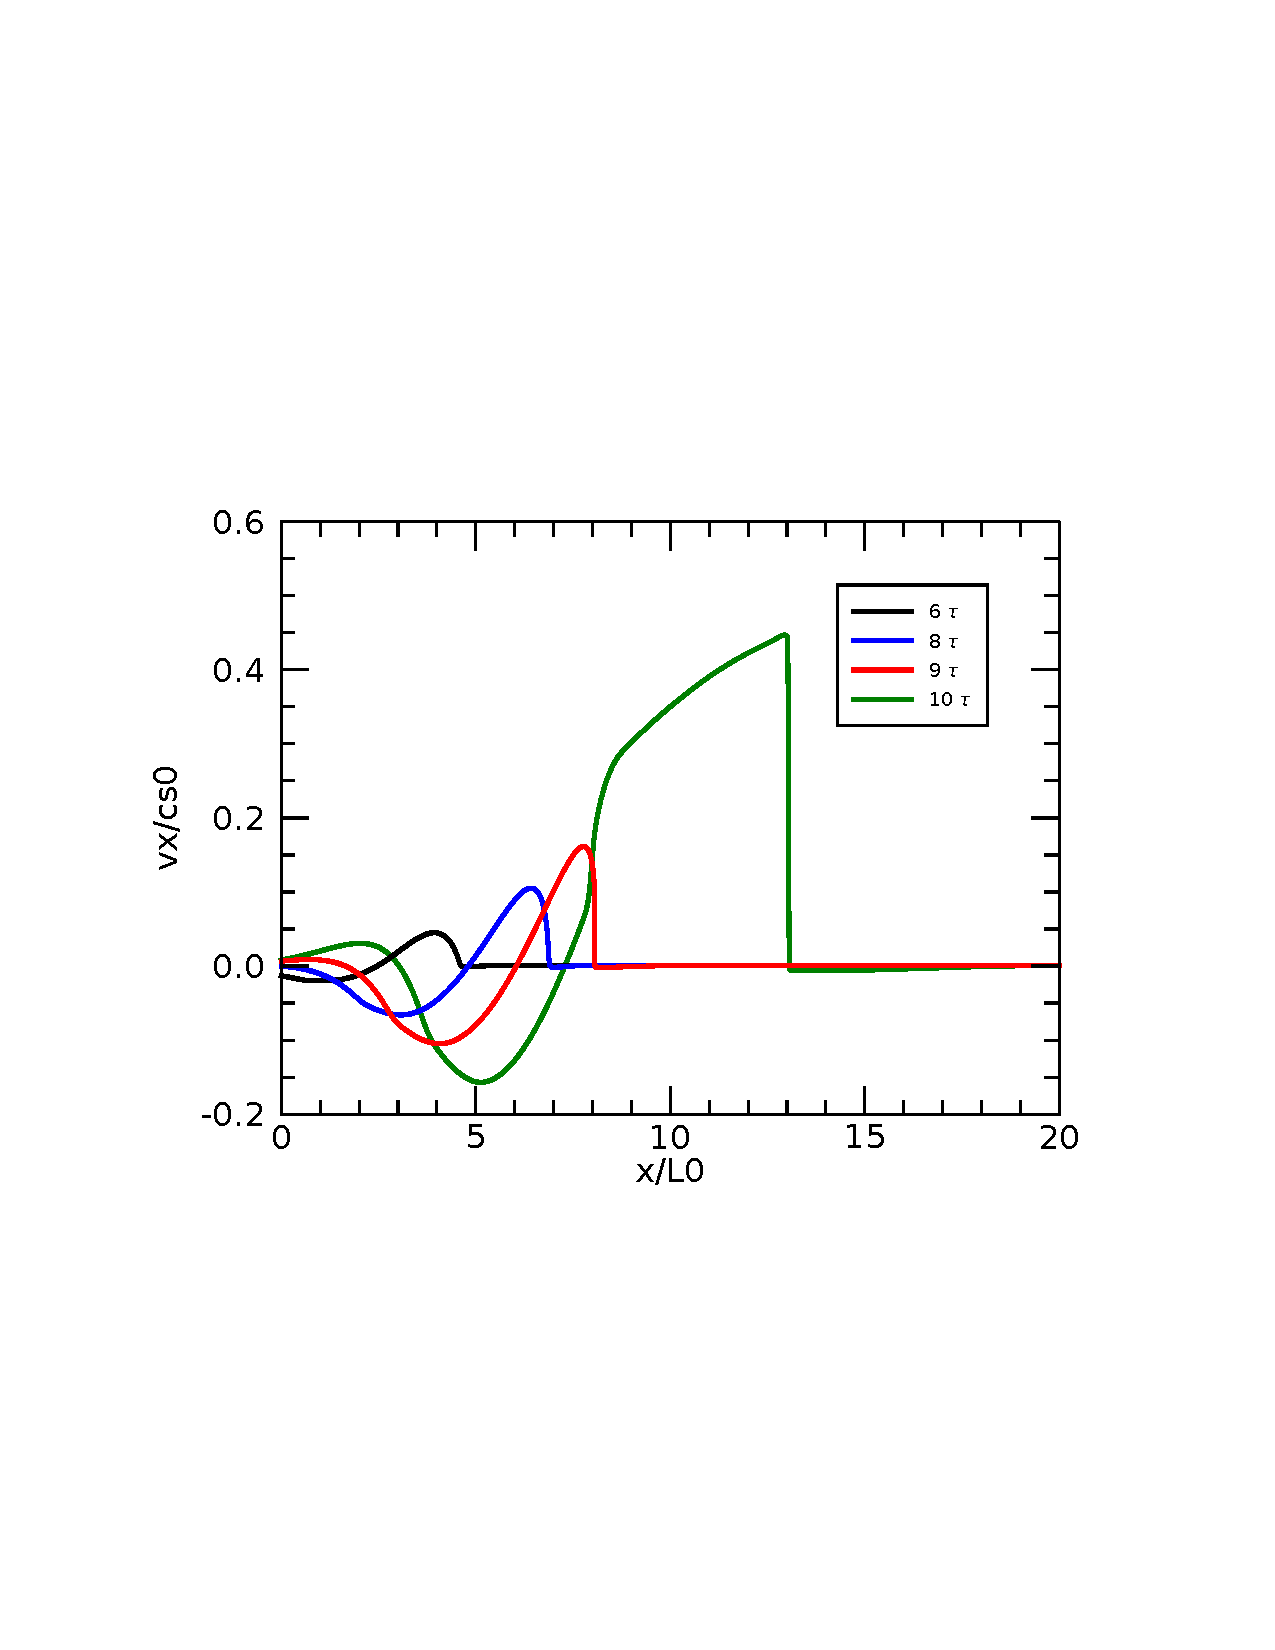
\includegraphics[width=0.95\textwidth, trim=2cm 7cm 2cm 8cm,clip]{2023ECRW/Figures/steepening.pdf} \\
%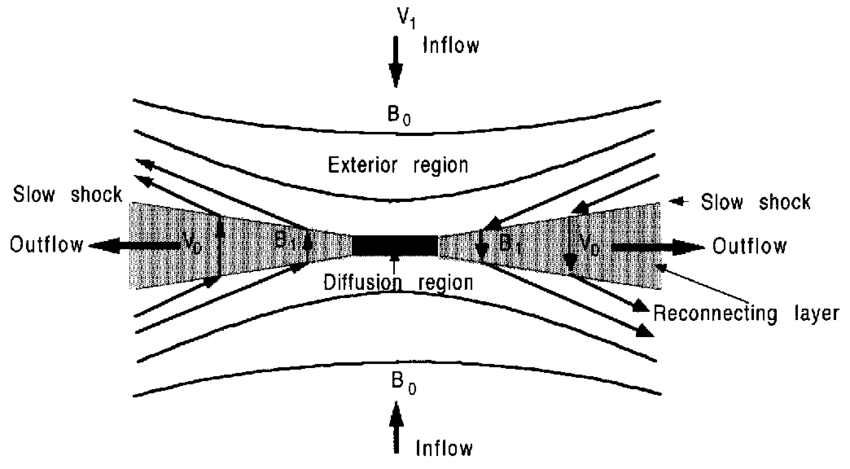
\includegraphics[width=0.95\linewidth]{2023RAS/Figures/petschek.png}
%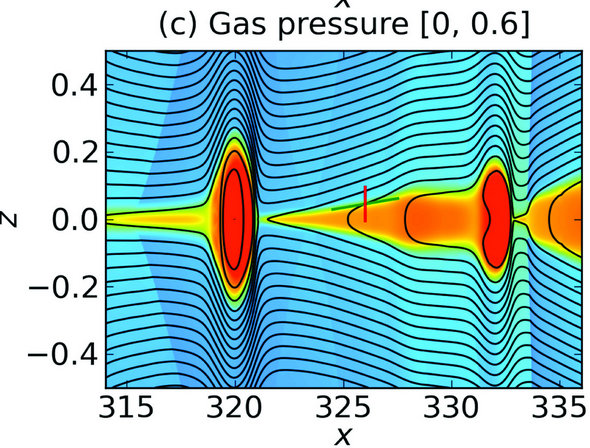
\includegraphics[width=0.95\linewidth]{2023RAS/Figures/shibyama.png}
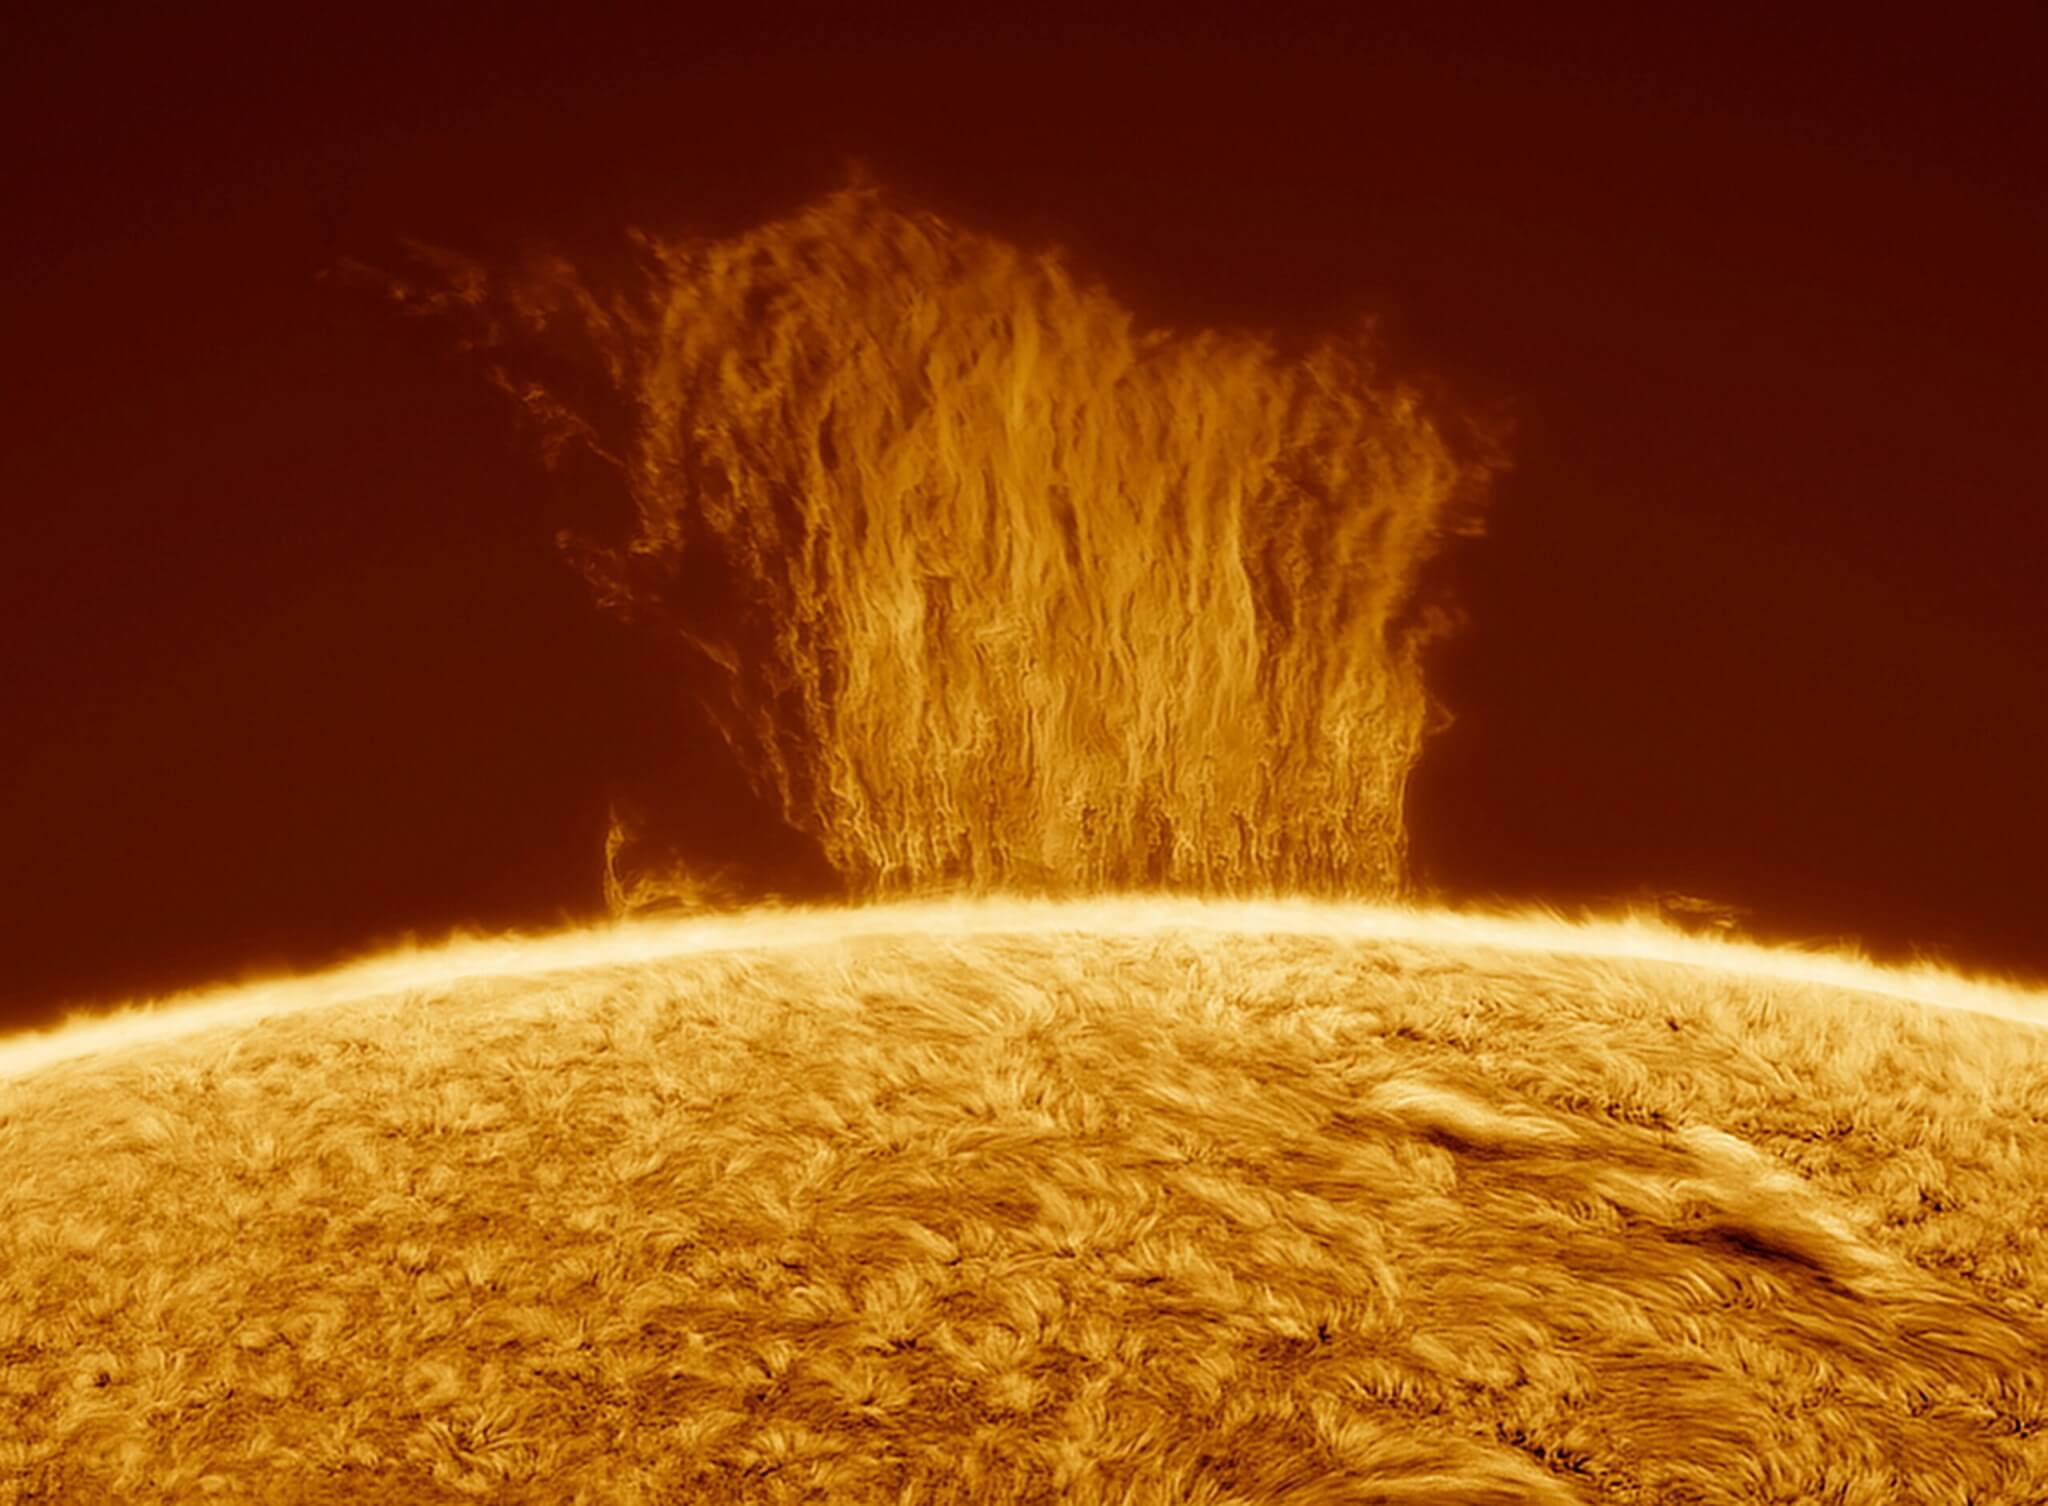
\includegraphics[width=0.9\linewidth]{2023Mixing/Figures/prominence.png}
\end{column}
\end{columns}
\end{frame}

% \begin{frame}{Ionisation states across the interface}
% \begin{columns}
% \begin{column}{0.5\textwidth}
% \begin{itemize}
%     \item Dense \& cool
%     \item Saha equations shows medium is partially ionised
%     \item Ions are MHD-like (directly affected by the magnetic field)
%     \item Neutrals are HD-like 
%     \item Partial ionisation is known to: speed up rate of magnetic reconnection, efficient damping of Alfv\'en waves, etc....
%     \item How does partial ionisation affect shocks?VALC
% \end{itemize}
% \end{column}
% \begin{column}{0.5\textwidth}
% \includegraphics[width=0.95\linewidth]{2023ECRW/Figures/saha2_plot.png}
% %\includegraphics[width=0.32\linewidth]{Figures/Crab_Nebula.jpeg}
% %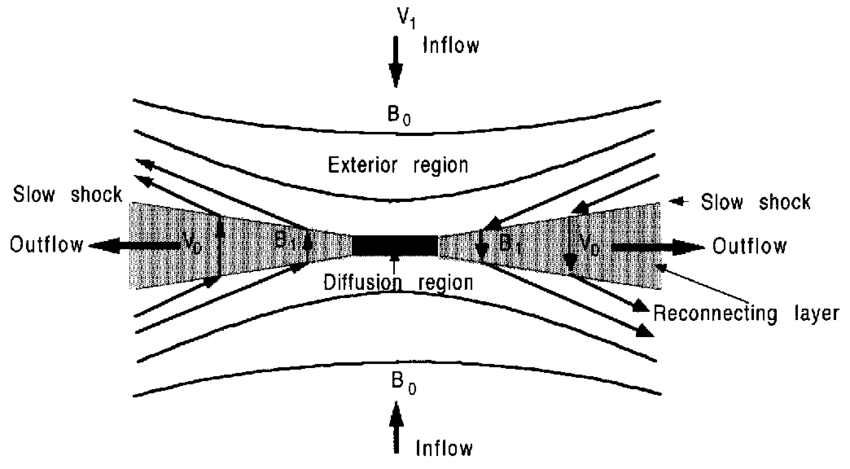
\includegraphics[width=0.95\linewidth]{2023RAS/Figures/petschek.png} \\
% %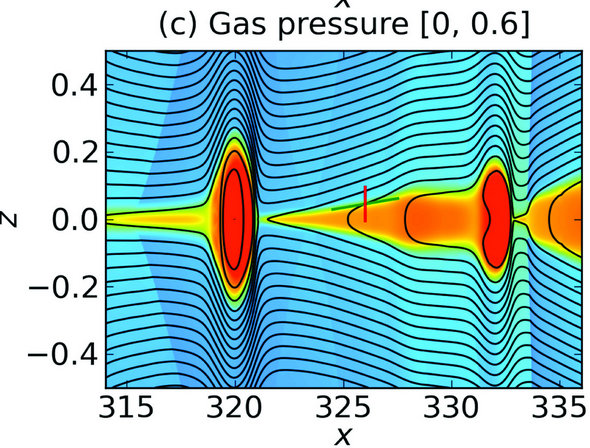
\includegraphics[width=0.95\linewidth]{2023RAS/Figures/shibyama.png}
% %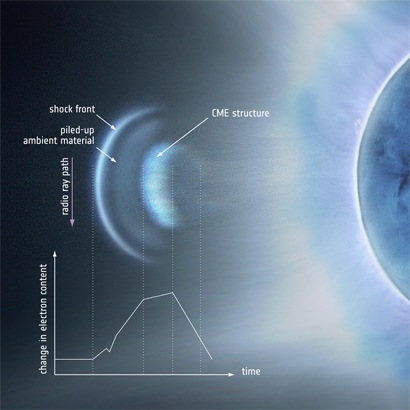
\includegraphics[width=0.32\linewidth]{Figures/cmesketch.jpg}
% \end{column}
% \end{columns}
% \end{frame}

\begin{frame}{Aims}
\begin{itemize}
    \item Multiple-level, non-equilibrium hydrogen model for ionisation/recombination using collsional/radiative rates in two-fluid framework.
    \item Study how KHI mixing behaves in partially-ionised systems (using collisional rates only)
    \item Structure of losses
\end{itemize}
\end{frame}

%%%%%%%%%%%%%%%%%%%%%%%%%%%%%%%%%%%%%%%%%%%%%%%%%%%%%%%%%%%%%%%%%%%%%%%%%%%%%%%%%%

\begin{frame}{Underlying equations}
\footnotesize
\begin{gather}
\frac{\partial \rho _{\text{n}}}{\partial t} + \nabla \cdot (\rho _{\text{n}} \textbf{v}_{\text{n}})= \Gamma _{rec} \rho _{\rm p} - \Gamma _{ion} \rho _{\rm n}, \label{eqn:neutral1}\tag{5} \\
\frac{\partial}{\partial t}(\rho _{\text{n}} \textbf{v}_{\text{n}}) + \nabla \cdot (\rho _{\text{n}} \textbf{v}_{\text{n}} \textbf{v}_{\text{n}} + P_{\text{n}} \textbf{I}) = -\alpha _c \rho_{\text{n}} \rho_{\text{p}} (\textbf{v}_{\text{n}}-\textbf{v}_{\text{p}}) + \Gamma _{rec} \rho _{\rm p} \textbf{v}_{\rm p} - \Gamma _{ion} \rho_{\rm n} \textbf{v}_{\rm n}, \tag{6}\\
\frac{\partial e_{\text{n}}}{\partial t} + \nabla \cdot \left[\textbf{v}_{\text{n}} (e_{\text{n}} +P_{\text{n}}) \right] = -\alpha _c \rho _{\text{n}} \rho _{\text{p}} \left[ \frac{1}{2} (\textbf{v}_{\text{n}} ^2 - \textbf{v}_{\text{p}} ^2)+ \frac{3}{2} \left(\frac{P_{\rm n}}{\rho_{\rm n}}-\frac{1}{2}\frac{P_{\rm p}}{\rho_{\rm p}}\right) \right] \nonumber \\ \hspace{0.5cm}+ \frac{1}{2} \left( \Gamma _{rec} \rho _{\rm p} \textbf{v}_{\rm p} ^2 - \Gamma _{ion} \rho _{\rm n} \textbf{v}_{\rm n} ^2 \right) +\frac{1}{ (\gamma-1)} \left( \frac{1}{2} \Gamma _{rec} P_{\rm p} -\Gamma _{ion} P_{\rm n} \right), \tag{7}\\
%e_{\text{n}} = \frac{P_{\text{n}}}{\gamma -1} + \frac{1}{2} \rho _{\text{n}} v_{\text{n}} ^2, \label{eqn:neutral2} \\
\frac{\partial \rho _{\text{p}}}{\partial t} + \nabla \cdot (\rho_{\text{p}} \textbf{v}_{\text{p}}) = - \Gamma _{rec} \rho _{\rm p} + \Gamma _{ion} \rho _{\rm n} \label{eqn:plasma1}\tag{8}\\
\frac{\partial}{\partial t} (\rho_{\text{p}} \textbf{v}_{\text{p}})+ \nabla \cdot \left( \rho_{\text{p}} \textbf{v}_{\text{p}} \textbf{v}_{\text{p}} + P_{\text{p}} \textbf{I} - \textbf{B B} + \frac{\textbf{B}^2}{2} \textbf{I} \right) = \alpha _c \rho_{\text{n}} \rho_{\text{p}}(\textbf{v}_{\text{n}} - \textbf{v}_{\text{p}}) - \Gamma _{rec} \rho _{\rm p} \textbf{v}_{\rm p} + \Gamma _{ion} \rho_{\rm n} \textbf{v}_{\rm n},\tag{9}\\
\frac{\partial}{\partial t} \left( e_{\text{p}} + \frac{\textbf{B}^2}{2} \right) + \nabla \cdot \left[ \textbf{v}_{\text{p}} ( e_{\text{p}} + P_{\text{p}}) -  (\textbf{v}_{\rm p} \times \textbf{B}) \times \textbf{B} \right]  =  \alpha _c \rho _{\text{n}} \rho _{\text{p}} \left[ \frac{1}{2} (\textbf{v}_{\text{n}} ^2 - \textbf{v}_{\text{p}} ^2)+ \frac{3}{2} \left(\frac{P_{\rm n}}{\rho_{\rm n}}-\frac{1}{2}\frac{P_{\rm p}}{\rho_{\rm p}}\right) \right] \nonumber \\ \hspace{0.5cm}- \frac{1}{2} \left( \Gamma _{rec} \rho _{\rm p} \textbf{v}_{\rm p} ^2 - \Gamma _{ion} \rho _{\rm n} \textbf{v}_{\rm n} ^2 \right) {- \phi_I + \phi_{heat}} -\frac{1}{ (\gamma-1)} \left( \frac{1}{2} \Gamma _{rec} P_{\rm p} -\Gamma _{ion} P_{\rm n} \right), \label{eqn:ep}\tag{10} \\
\frac{\partial \textbf{B}}{\partial t} - \nabla \times (\textbf{v}_{\text{p}} \times \textbf{B}) = 0.\tag{11}
%e_{\text{p}} = \frac{P_{\text{p}}}{\gamma -1} + \frac{1}{2} \rho _{\text{p}} v_{\text{p}} ^2, \\
%\nabla \cdot \textbf{B} = 0,\label{eqn:plasma2}
\end{gather}
\end{frame}

\begin{frame}{Underlying equations}
\vspace{-0.5cm}
\footnotesize
\begin{gather}
\mathcolorbox{VioletRed}{\frac{\partial \rho _{\text{n}}}{\partial t} + \nabla \cdot (\rho _{\text{n}} \textbf{v}_{\text{n}})}= \Gamma _{rec} \rho _{\rm p} - \Gamma _{ion} \rho _{\rm n}, \label{eqn:neutral1}\tag{5} \\
\mathcolorbox{VioletRed}{\frac{\partial}{\partial t}(\rho _{\text{n}} \textbf{v}_{\text{n}}) + \nabla \cdot (\rho _{\text{n}} \textbf{v}_{\text{n}} \textbf{v}_{\text{n}} + P_{\text{n}} \textbf{I})} = -\alpha _c \rho_{\text{n}} \rho_{\text{p}} (\textbf{v}_{\text{n}}-\textbf{v}_{\text{p}}) + \Gamma _{rec} \rho _{\rm p} \textbf{v}_{\rm p} - \Gamma _{ion} \rho_{\rm n} \textbf{v}_{\rm n}, \tag{6}\\
\mathcolorbox{VioletRed}{\frac{\partial e_{\text{n}}}{\partial t} + \nabla \cdot \left[\textbf{v}_{\text{n}} (e_{\text{n}} +P_{\text{n}}) \right]} = -\alpha _c \rho _{\text{n}} \rho _{\text{p}} \left[ \frac{1}{2} (\textbf{v}_{\text{n}} ^2 - \textbf{v}_{\text{p}} ^2)+ \frac{3}{2} \left(\frac{P_{\rm n}}{\rho_{\rm n}}-\frac{1}{2}\frac{P_{\rm p}}{\rho_{\rm p}}\right) \right] \nonumber \\ \hspace{0.5cm}+ \frac{1}{2} \left( \Gamma _{rec} \rho _{\rm p} \textbf{v}_{\rm p} ^2 - \Gamma _{ion} \rho _{\rm n} \textbf{v}_{\rm n} ^2 \right) +\frac{1}{ (\gamma-1)} \left( \frac{1}{2} \Gamma _{rec} P_{\rm p} -\Gamma _{ion} P_{\rm n} \right), \tag{7}\\
%e_{\text{n}} = \frac{P_{\text{n}}}{\gamma -1} + \frac{1}{2} \rho _{\text{n}} v_{\text{n}} ^2, \label{eqn:neutral2} \\
\frac{\partial \rho _{\text{p}}}{\partial t} + \nabla \cdot (\rho_{\text{p}} \textbf{v}_{\text{p}}) = - \Gamma _{rec} \rho _{\rm p} + \Gamma _{ion} \rho _{\rm n} \label{eqn:plasma1}\tag{8}\\
\frac{\partial}{\partial t} (\rho_{\text{p}} \textbf{v}_{\text{p}})+ \nabla \cdot \left( \rho_{\text{p}} \textbf{v}_{\text{p}} \textbf{v}_{\text{p}} + P_{\text{p}} \textbf{I} - \textbf{B B} + \frac{\textbf{B}^2}{2} \textbf{I} \right) = \alpha _c \rho_{\text{n}} \rho_{\text{p}}(\textbf{v}_{\text{n}} - \textbf{v}_{\text{p}}) - \Gamma _{rec} \rho _{\rm p} \textbf{v}_{\rm p} + \Gamma _{ion} \rho_{\rm n} \textbf{v}_{\rm n},\tag{9}\\
\frac{\partial}{\partial t} \left( e_{\text{p}} + \frac{\textbf{B}^2}{2} \right) + \nabla \cdot \left[ \textbf{v}_{\text{p}} ( e_{\text{p}} + P_{\text{p}}) -  (\textbf{v}_{\rm p} \times \textbf{B}) \times \textbf{B} \right]  =  \alpha _c \rho _{\text{n}} \rho _{\text{p}} \left[ \frac{1}{2} (\textbf{v}_{\text{n}} ^2 - \textbf{v}_{\text{p}} ^2)+ \frac{3}{2} \left(\frac{P_{\rm n}}{\rho_{\rm n}}-\frac{1}{2}\frac{P_{\rm p}}{\rho_{\rm p}}\right) \right] \nonumber \\ \hspace{0.5cm}- \frac{1}{2} \left( \Gamma _{rec} \rho _{\rm p} \textbf{v}_{\rm p} ^2 - \Gamma _{ion} \rho _{\rm n} \textbf{v}_{\rm n} ^2 \right) {- \phi_I + \phi_{heat}} -\frac{1}{ (\gamma-1)} \left( \frac{1}{2} \Gamma _{rec} P_{\rm p} -\Gamma _{ion} P_{\rm n} \right), \label{eqn:ep} \tag{10}\\
\frac{\partial \textbf{B}}{\partial t} - \nabla \times (\textbf{v}_{\text{p}} \times \textbf{B}) = 0.\tag{11}
%e_{\text{p}} = \frac{P_{\text{p}}}{\gamma -1} + \frac{1}{2} \rho _{\text{p}} v_{\text{p}} ^2, \\
%\nabla \cdot \textbf{B} = 0,\label{eqn:plasma2}
\end{gather}
\end{frame}

\begin{frame}{Underlying equations}
\vspace{-0.5cm}
\footnotesize
\begin{gather}
\frac{\partial \rho _{\text{n}}}{\partial t} + \nabla \cdot (\rho _{\text{n}} \textbf{v}_{\text{n}})= \Gamma _{rec} \rho _{\rm p} - \Gamma _{ion} \rho _{\rm n}, \label{eqn:neutral1}\tag{5} \\
\frac{\partial}{\partial t}(\rho _{\text{n}} \textbf{v}_{\text{n}}) + \nabla \cdot (\rho _{\text{n}} \textbf{v}_{\text{n}} \textbf{v}_{\text{n}} + P_{\text{n}} \textbf{I}) = -\alpha _c \rho_{\text{n}} \rho_{\text{p}} (\textbf{v}_{\text{n}}-\textbf{v}_{\text{p}}) + \Gamma _{rec} \rho _{\rm p} \textbf{v}_{\rm p} - \Gamma _{ion} \rho_{\rm n} \textbf{v}_{\rm n}, \tag{6}\\
\frac{\partial e_{\text{n}}}{\partial t} + \nabla \cdot \left[\textbf{v}_{\text{n}} (e_{\text{n}} +P_{\text{n}}) \right] = -\alpha _c \rho _{\text{n}} \rho _{\text{p}} \left[ \frac{1}{2} (\textbf{v}_{\text{n}} ^2 - \textbf{v}_{\text{p}} ^2)+ \frac{3}{2} \left(\frac{P_{\rm n}}{\rho_{\rm n}}-\frac{1}{2}\frac{P_{\rm p}}{\rho_{\rm p}}\right) \right] \nonumber \\ \hspace{0.5cm}+ \frac{1}{2} \left( \Gamma _{rec} \rho _{\rm p} \textbf{v}_{\rm p} ^2 - \Gamma _{ion} \rho _{\rm n} \textbf{v}_{\rm n} ^2 \right) +\frac{1}{ (\gamma-1)} \left( \frac{1}{2} \Gamma _{rec} P_{\rm p} -\Gamma _{ion} P_{\rm n} \right), \tag{7}\\
%e_{\text{n}} = \frac{P_{\text{n}}}{\gamma -1} + \frac{1}{2} \rho _{\text{n}} v_{\text{n}} ^2, \label{eqn:neutral2} \\
\mathcolorbox{BlueGreen}{\frac{\partial \rho _{\text{p}}}{\partial t} + \nabla \cdot (\rho_{\text{p}} \textbf{v}_{\text{p}})} = - \Gamma _{rec} \rho _{\rm p} + \Gamma _{ion} \rho _{\rm n} \label{eqn:plasma1}\tag{8}\\
\mathcolorbox{BlueGreen}{\frac{\partial}{\partial t} (\rho_{\text{p}} \textbf{v}_{\text{p}})+ \nabla \cdot \left( \rho_{\text{p}} \textbf{v}_{\text{p}} \textbf{v}_{\text{p}} + P_{\text{p}} \textbf{I} - \textbf{B B} + \frac{\textbf{B}^2}{2} \textbf{I} \right)} = \alpha _c \rho_{\text{n}} \rho_{\text{p}}(\textbf{v}_{\text{n}} - \textbf{v}_{\text{p}}) - \Gamma _{rec} \rho _{\rm p} \textbf{v}_{\rm p} + \Gamma _{ion} \rho_{\rm n} \textbf{v}_{\rm n},\tag{9}\\
\mathcolorbox{BlueGreen}{\frac{\partial}{\partial t} \left( e_{\text{p}} + \frac{\textbf{B}^2}{2} \right) + \nabla \cdot \left[ \textbf{v}_{\text{p}} ( e_{\text{p}} + P_{\text{p}}) -  (\textbf{v}_{\rm p} \times \textbf{B}) \times \textbf{B} \right] } =  \alpha _c \rho _{\text{n}} \rho _{\text{p}} \left[ \frac{1}{2} (\textbf{v}_{\text{n}} ^2 - \textbf{v}_{\text{p}} ^2)+ \frac{3}{2} \left(\frac{P_{\rm n}}{\rho_{\rm n}}-\frac{1}{2}\frac{P_{\rm p}}{\rho_{\rm p}}\right) \right] \nonumber \\ \hspace{0.5cm}- \frac{1}{2} \left( \Gamma _{rec} \rho _{\rm p} \textbf{v}_{\rm p} ^2 - \Gamma _{ion} \rho _{\rm n} \textbf{v}_{\rm n} ^2 \right) {- \phi_I + \phi_{heat}} -\frac{1}{ (\gamma-1)} \left( \frac{1}{2} \Gamma _{rec} P_{\rm p} -\Gamma _{ion} P_{\rm n} \right), \label{eqn:ep}\tag{10} \\
\mathcolorbox{BlueGreen}{\frac{\partial \textbf{B}}{\partial t} - \nabla \times (\textbf{v}_{\text{p}} \times \textbf{B}) = 0.}\tag{11}
%e_{\text{p}} = \frac{P_{\text{p}}}{\gamma -1} + \frac{1}{2} \rho _{\text{p}} v_{\text{p}} ^2, \\
%\nabla \cdot \textbf{B} = 0,\label{eqn:plasma2}
\end{gather}
\end{frame}

\begin{frame}{Underlying equations}
\vspace{-0.5cm}
\footnotesize
\begin{gather}
\frac{\partial \rho _{\text{n}}}{\partial t} + \nabla \cdot (\rho _{\text{n}} \textbf{v}_{\text{n}})= \Gamma _{rec} \rho _{\rm p} - \Gamma _{ion} \rho _{\rm n}, \label{eqn:neutral1}\tag{5} \\
\frac{\partial}{\partial t}(\rho _{\text{n}} \textbf{v}_{\text{n}}) + \nabla \cdot (\rho _{\text{n}} \textbf{v}_{\text{n}} \textbf{v}_{\text{n}} + P_{\text{n}} \textbf{I}) =\mathcolorbox{YellowOrange}{ -\alpha _c \rho_{\text{n}} \rho_{\text{p}} (\textbf{v}_{\text{n}}-\textbf{v}_{\text{p}})} + \Gamma _{rec} \rho _{\rm p} \textbf{v}_{\rm p} - \Gamma _{ion} \rho_{\rm n} \textbf{v}_{\rm n}, \tag{6}\\
\frac{\partial e_{\text{n}}}{\partial t} + \nabla \cdot \left[\textbf{v}_{\text{n}} (e_{\text{n}} +P_{\text{n}}) \right] = \mathcolorbox{YellowOrange}{-\alpha _c \rho _{\text{n}} \rho _{\text{p}} \left[ \frac{1}{2} (\textbf{v}_{\text{n}} ^2 - \textbf{v}_{\text{p}} ^2)+ \frac{3}{2} \left(\frac{P_{\rm n}}{\rho_{\rm n}}-\frac{1}{2}\frac{P_{\rm p}}{\rho_{\rm p}}\right) \right]} \nonumber \\ \hspace{0.5cm}+ \frac{1}{2} \left( \Gamma _{rec} \rho _{\rm p} \textbf{v}_{\rm p} ^2 - \Gamma _{ion} \rho _{\rm n} \textbf{v}_{\rm n} ^2 \right) +\frac{1}{ (\gamma-1)} \left( \frac{1}{2} \Gamma _{rec} P_{\rm p} -\Gamma _{ion} P_{\rm n} \right), \tag{7}\\
%e_{\text{n}} = \frac{P_{\text{n}}}{\gamma -1} + \frac{1}{2} \rho _{\text{n}} v_{\text{n}} ^2, \label{eqn:neutral2} \\
\frac{\partial \rho _{\text{p}}}{\partial t} + \nabla \cdot (\rho_{\text{p}} \textbf{v}_{\text{p}}) = - \Gamma _{rec} \rho _{\rm p} + \Gamma _{ion} \rho _{\rm n} \label{eqn:plasma1}\tag{8}\\
\frac{\partial}{\partial t} (\rho_{\text{p}} \textbf{v}_{\text{p}})+ \nabla \cdot \left( \rho_{\text{p}} \textbf{v}_{\text{p}} \textbf{v}_{\text{p}} + P_{\text{p}} \textbf{I} - \textbf{B B} + \frac{\textbf{B}^2}{2} \textbf{I} \right) = \mathcolorbox{YellowOrange}{\alpha _c \rho_{\text{n}} \rho_{\text{p}}(\textbf{v}_{\text{n}} - \textbf{v}_{\text{p}})} - \Gamma _{rec} \rho _{\rm p} \textbf{v}_{\rm p} + \Gamma _{ion} \rho_{\rm n} \textbf{v}_{\rm n},\tag{9}\\
\frac{\partial}{\partial t} \left( e_{\text{p}} + \frac{\textbf{B}^2}{2} \right) + \nabla \cdot \left[ \textbf{v}_{\text{p}} ( e_{\text{p}} + P_{\text{p}}) -  (\textbf{v}_{\rm p} \times \textbf{B}) \times \textbf{B} \right]  = \mathcolorbox{YellowOrange}{ \alpha _c \rho _{\text{n}} \rho _{\text{p}} \left[ \frac{1}{2} (\textbf{v}_{\text{n}} ^2 - \textbf{v}_{\text{p}} ^2)+ \frac{3}{2} \left(\frac{P_{\rm n}}{\rho_{\rm n}}-\frac{1}{2}\frac{P_{\rm p}}{\rho_{\rm p}}\right) \right]} \nonumber \\ \hspace{0.5cm}- \frac{1}{2} \left( \Gamma _{rec} \rho _{\rm p} \textbf{v}_{\rm p} ^2 - \Gamma _{ion} \rho _{\rm n} \textbf{v}_{\rm n} ^2 \right) {- \phi_I + \phi_{heat}} -\frac{1}{ (\gamma-1)} \left( \frac{1}{2} \Gamma _{rec} P_{\rm p} -\Gamma _{ion} P_{\rm n} \right), \label{eqn:ep} \tag{10}\\
\frac{\partial \textbf{B}}{\partial t} - \nabla \times (\textbf{v}_{\text{p}} \times \textbf{B}) = 0.\tag{11}
%e_{\text{p}} = \frac{P_{\text{p}}}{\gamma -1} + \frac{1}{2} \rho _{\text{p}} v_{\text{p}} ^2, \\
%\nabla \cdot \textbf{B} = 0,\label{eqn:plasma2}
\end{gather}
\end{frame}

\begin{frame}{Underlying equations}
\vspace{-0.5cm}
\footnotesize
\begin{gather}
\frac{\partial \rho _{\text{n}}}{\partial t} + \nabla \cdot (\rho _{\text{n}} \textbf{v}_{\text{n}})= \mathcolorbox{LimeGreen}{\Gamma _{rec} \rho _{\rm p} - \Gamma _{ion} \rho _{\rm n},} \label{eqn:neutral1}\tag{5} \\
\frac{\partial}{\partial t}(\rho _{\text{n}} \textbf{v}_{\text{n}}) + \nabla \cdot (\rho _{\text{n}} \textbf{v}_{\text{n}} \textbf{v}_{\text{n}} + P_{\text{n}} \textbf{I}) = -\alpha _c \rho_{\text{n}} \rho_{\text{p}} (\textbf{v}_{\text{n}}-\textbf{v}_{\text{p}}) + \mathcolorbox{LimeGreen}{\Gamma _{rec} \rho _{\rm p} \textbf{v}_{\rm p} - \Gamma _{ion} \rho_{\rm n} \textbf{v}_{\rm n}}, \tag{6}\\
\frac{\partial e_{\text{n}}}{\partial t} + \nabla \cdot \left[\textbf{v}_{\text{n}} (e_{\text{n}} +P_{\text{n}}) \right] = -\alpha _c \rho _{\text{n}} \rho _{\text{p}} \left[ \frac{1}{2} (\textbf{v}_{\text{n}} ^2 - \textbf{v}_{\text{p}} ^2)+ \frac{3}{2} \left(\frac{P_{\rm n}}{\rho_{\rm n}}-\frac{1}{2}\frac{P_{\rm p}}{\rho_{\rm p}}\right) \right] \nonumber \\ \hspace{0.5cm}+ \mathcolorbox{LimeGreen}{\frac{1}{2} \left( \Gamma _{rec} \rho _{\rm p} \textbf{v}_{\rm p} ^2 - \Gamma _{ion} \rho _{\rm n} \textbf{v}_{\rm n} ^2 \right) +\frac{1}{ (\gamma-1)} \left( \frac{1}{2} \Gamma _{rec} P_{\rm p} -\Gamma _{ion} P_{\rm n} \right),} \tag{7}\\
%e_{\text{n}} = \frac{P_{\text{n}}}{\gamma -1} + \frac{1}{2} \rho _{\text{n}} v_{\text{n}} ^2, \label{eqn:neutral2} \\
\frac{\partial \rho _{\text{p}}}{\partial t} + \nabla \cdot (\rho_{\text{p}} \textbf{v}_{\text{p}}) = \mathcolorbox{LimeGreen}{- \Gamma _{rec} \rho _{\rm p} + \Gamma _{ion} \rho _{\rm n}} \label{eqn:plasma1}\tag{8}\\
\frac{\partial}{\partial t} (\rho_{\text{p}} \textbf{v}_{\text{p}})+ \nabla \cdot \left( \rho_{\text{p}} \textbf{v}_{\text{p}} \textbf{v}_{\text{p}} + P_{\text{p}} \textbf{I} - \textbf{B B} + \frac{\textbf{B}^2}{2} \textbf{I} \right) = \alpha _c \rho_{\text{n}} \rho_{\text{p}}(\textbf{v}_{\text{n}} - \textbf{v}_{\text{p}}) \mathcolorbox{LimeGreen}{- \Gamma _{rec} \rho _{\rm p} \textbf{v}_{\rm p} + \Gamma _{ion} \rho_{\rm n} \textbf{v}_{\rm n},}\tag{9}\\
\frac{\partial}{\partial t} \left( e_{\text{p}} + \frac{\textbf{B}^2}{2} \right) + \nabla \cdot \left[ \textbf{v}_{\text{p}} ( e_{\text{p}} + P_{\text{p}}) -  (\textbf{v}_{\rm p} \times \textbf{B}) \times \textbf{B} \right]  =  \alpha _c \rho _{\text{n}} \rho _{\text{p}} \left[ \frac{1}{2} (\textbf{v}_{\text{n}} ^2 - \textbf{v}_{\text{p}} ^2)+ \frac{3}{2} \left(\frac{P_{\rm n}}{\rho_{\rm n}}-\frac{1}{2}\frac{P_{\rm p}}{\rho_{\rm p}}\right) \right] \nonumber \\ \hspace{0.5cm}\mathcolorbox{LimeGreen}{- \frac{1}{2} \left( \Gamma _{rec} \rho _{\rm p} \textbf{v}_{\rm p} ^2 - \Gamma _{ion} \rho _{\rm n} \textbf{v}_{\rm n} ^2 \right)} {- \phi_I + \phi_{heat}} \mathcolorbox{LimeGreen}{-\frac{1}{ (\gamma-1)} \left( \frac{1}{2} \Gamma _{rec} P_{\rm p} -\Gamma _{ion} P_{\rm n} \right)}, \label{eqn:ep} \tag{10}\\
\frac{\partial \textbf{B}}{\partial t} - \nabla \times (\textbf{v}_{\text{p}} \times \textbf{B}) = 0.\tag{11}
%e_{\text{p}} = \frac{P_{\text{p}}}{\gamma -1} + \frac{1}{2} \rho _{\text{p}} v_{\text{p}} ^2, \\
%\nabla \cdot \textbf{B} = 0,\label{eqn:plasma2}
\end{gather}
\end{frame}

% \begin{frame}{Ionisation/recombination model}
% \begin{columns}
% \begin{column}{0.3\textwidth}
% \begin{itemize}
% %\item Two-fluid model - ion+electron plasma, and bulk neutral fluid.
% \item 5 levels of neutral hydrogen + continuum/ionised plasma.
% \item Assume all neutral hydrogen levels move as one.
% \item Optically thick approximation for Lyman transitions.
% \item Leenaarts+2007, Johnson1972, Sollum1999
% \end{itemize}
% \end{column}
% \begin{column}{0.7\textwidth}
% \begin{gather}
%     % \Gamma_{\rm rec} \rho_{\rm p} = \rho_{\rm p} (C_{\rm{p},1}+C_{\rm{p},2}+C_{\rm{p},3}+C_{\rm{p},4}+C_{\rm{p},5}) \nonumber \\
%     %     \hspace{2cm}+ \rho_{\rm{p}} (R_{\rm{p},1}+R_{\rm{p},2}+R_{\rm{p},3}+R_{\rm{p},4}+R_{\rm{p},5}) \\
%     %     \hspace{1.4cm} = \rho_p \Gamma_{\rm rec,c} + \rho_p \Gamma_{\rm rec,r}
%     \Gamma_{\rm rec} \rho_{\rm p} = \rho_{\rm p} (\hat{C}_{\rm{p},1}+\hat{C}_{\rm{p},2}+\hat{C}_{\rm{p},3}+\hat{C}_{\rm{p},4}+\hat{C}_{\rm{p},5})/\hat{\Gamma} \nonumber \\
%         \hspace{1.2cm}+ \rho_{\rm{p}} (\hat{R}_{\rm{p},1}+\hat{R}_{\rm{p},2}+\hat{R}_{\rm{p},3}+\hat{R}_{\rm{p},4}+\hat{R}_{\rm{p},5})/\hat{\Gamma} \nonumber \\
%         \hspace{1.2cm} = \rho_{\rm p} (\hat{\Gamma}_{\rm rec,col} + \hat{\Gamma}_{\rm rec,rec})/\hat{\Gamma} \nonumber
% \end{gather}
% \begin{gather}
%     \Gamma_{\rm ion} \rho_{\rm{n}} = (\rho_{\rm{n}1} \hat{C}_{1,\rm{p}}+\rho_{n2}\hat{C}_{2,\rm{p}}+\rho_{\rm{n}3}\hat{C}_{3,\rm{p}}+\rho_{\rm{n}4}\hat{C}_{4,\rm{p}}+\rho_{\rm{n}5}\hat{C}_{5,\rm{p}})/\hat{\Gamma} \nonumber \\  
%     \hspace{1cm}+(\rho_{\rm{n}1}\hat{R}_{1,\rm{p}}+\rho_{\rm{n}2}\hat{R}_{2,\rm{p}}+\rho_{\rm{n}3} \hat{R}_{3,\rm{p}}+\rho_{\rm{n}4}\hat{R}_{4,\rm{p}}+\rho_{\rm{n}5}\hat{R}_{5,\rm{p}})/\hat{\Gamma}  \nonumber\\
%     \hspace{1cm} = \rho_{\rm{n}} (\hat{\Gamma}_{\rm ion,col} + \hat{\Gamma}_{\rm ion,rad})/\hat{\Gamma} \nonumber
% \end{gather}
% \end{column}
% \end{columns}
% \end{frame}

\begin{frame}{Underlying equations}
\footnotesize
\begin{gather}
\frac{\partial \rho _{\text{n}}}{\partial t} + \nabla \cdot (\rho _{\text{n}} \textbf{v}_{\text{n}})= \Gamma _{rec} \rho _{\rm p} - \Gamma _{ion} \rho _{\rm n}, \label{eqn:neutral1}\tag{5} \\
\frac{\partial}{\partial t}(\rho _{\text{n}} \textbf{v}_{\text{n}}) + \nabla \cdot (\rho _{\text{n}} \textbf{v}_{\text{n}} \textbf{v}_{\text{n}} + P_{\text{n}} \textbf{I}) = -\alpha _c \rho_{\text{n}} \rho_{\text{p}} (\textbf{v}_{\text{n}}-\textbf{v}_{\text{p}}) + \Gamma _{rec} \rho _{\rm p} \textbf{v}_{\rm p} - \Gamma _{ion} \rho_{\rm n} \textbf{v}_{\rm n},\tag{6} \\
\frac{\partial e_{\text{n}}}{\partial t} + \nabla \cdot \left[\textbf{v}_{\text{n}} (e_{\text{n}} +P_{\text{n}}) \right] = -\alpha _c \rho _{\text{n}} \rho _{\text{p}} \left[ \frac{1}{2} (\textbf{v}_{\text{n}} ^2 - \textbf{v}_{\text{p}} ^2)+ \frac{3}{2} \left(\frac{P_{\rm n}}{\rho_{\rm n}}-\frac{1}{2}\frac{P_{\rm p}}{\rho_{\rm p}}\right) \right] \nonumber \\ \hspace{0.5cm}+ \frac{1}{2} \left( \Gamma _{rec} \rho _{\rm p} \textbf{v}_{\rm p} ^2 - \Gamma _{ion} \rho _{\rm n} \textbf{v}_{\rm n} ^2 \right) +\frac{1}{ (\gamma-1)} \left( \frac{1}{2} \Gamma _{rec} P_{\rm p} -\Gamma _{ion} P_{\rm n} \right), \tag{7}\\
%e_{\text{n}} = \frac{P_{\text{n}}}{\gamma -1} + \frac{1}{2} \rho _{\text{n}} v_{\text{n}} ^2, \label{eqn:neutral2} \\
\frac{\partial \rho _{\text{p}}}{\partial t} + \nabla \cdot (\rho_{\text{p}} \textbf{v}_{\text{p}}) = - \Gamma _{rec} \rho _{\rm p} + \Gamma _{ion} \rho _{\rm n} \label{eqn:plasma1}\tag{8}\\
\frac{\partial}{\partial t} (\rho_{\text{p}} \textbf{v}_{\text{p}})+ \nabla \cdot \left( \rho_{\text{p}} \textbf{v}_{\text{p}} \textbf{v}_{\text{p}} + P_{\text{p}} \textbf{I} - \textbf{B B} + \frac{\textbf{B}^2}{2} \textbf{I} \right) = \alpha _c \rho_{\text{n}} \rho_{\text{p}}(\textbf{v}_{\text{n}} - \textbf{v}_{\text{p}}) - \Gamma _{rec} \rho _{\rm p} \textbf{v}_{\rm p} + \Gamma _{ion} \rho_{\rm n} \textbf{v}_{\rm n},\tag{9}\\
\frac{\partial}{\partial t} \left( e_{\text{p}} + \frac{\textbf{B}^2}{2} \right) + \nabla \cdot \left[ \textbf{v}_{\text{p}} ( e_{\text{p}} + P_{\text{p}}) -  (\textbf{v}_{\rm p} \times \textbf{B}) \times \textbf{B} \right]  =  \alpha _c \rho _{\text{n}} \rho _{\text{p}} \left[ \frac{1}{2} (\textbf{v}_{\text{n}} ^2 - \textbf{v}_{\text{p}} ^2)+ \frac{3}{2} \left(\frac{P_{\rm n}}{\rho_{\rm n}}-\frac{1}{2}\frac{P_{\rm p}}{\rho_{\rm p}}\right) \right] \nonumber \\ \hspace{0.5cm}- \frac{1}{2} \left( \Gamma _{rec} \rho _{\rm p} \textbf{v}_{\rm p} ^2 - \Gamma _{ion} \rho _{\rm n} \textbf{v}_{\rm n} ^2 \right) \mathcolorbox{yellow}{- \phi_I + \phi_{heat}} -\frac{1}{ (\gamma-1)} \left( \frac{1}{2} \Gamma _{rec} P_{\rm p} -\Gamma _{ion} P_{\rm n} \right), \label{eqn:ep} \tag{10}\\
\frac{\partial \textbf{B}}{\partial t} - \nabla \times (\textbf{v}_{\text{p}} \times \textbf{B}) = 0.\tag{11}
%e_{\text{p}} = \frac{P_{\text{p}}}{\gamma -1} + \frac{1}{2} \rho _{\text{p}} v_{\text{p}} ^2, \\
%\nabla \cdot \textbf{B} = 0,\label{eqn:plasma2}
\end{gather}
\end{frame}

\begin{frame}{Energies of the system}
\begin{columns}
\begin{column}{0.3\textwidth}
\centering
\textbf{Macroscopic fluid energy}
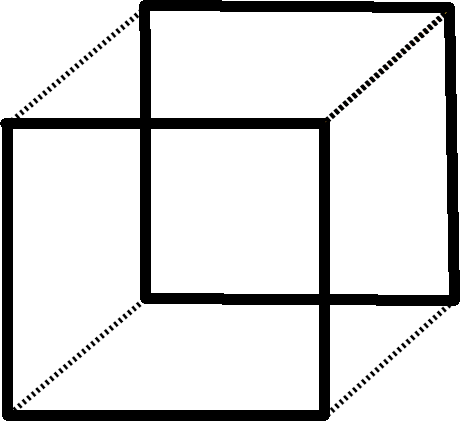
\includegraphics[width=0.9\textwidth]{2023ECRW/Figures/fluidelement.png}
\begin{itemize}
    \item Directly modelled
    \item Kinetic, Magnetic, thermal
\end{itemize}
\end{column}
\begin{column}{0.3\textwidth}
\centering
\textbf{Ionisation/excitation energy}
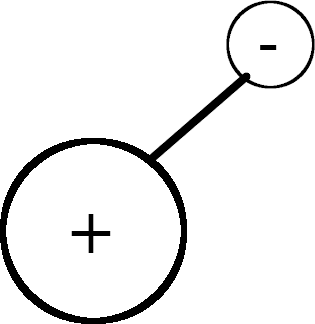
\includegraphics[width=0.8\textwidth]{2023ECRW/Figures/ionenergy.png}
\begin{itemize}
    \item Not directly modelled but can be calculated
    \item Non-conservative 
    \item Energy remains 'in the system'.
\end{itemize}
\end{column}
\begin{column}{0.3\textwidth}
\centering
\textbf{Energy loss terms}
\begin{gather}
    % \Gamma_{\rm rec} \rho_{\rm p} = \rho_{\rm p} (C_{\rm{p},1}+C_{\rm{p},2}+C_{\rm{p},3}+C_{\rm{p},4}+C_{\rm{p},5}) \nonumber \\
    %     \hspace{2cm}+ \rho_{\rm{p}} (R_{\rm{p},1}+R_{\rm{p},2}+R_{\rm{p},3}+R_{\rm{p},4}+R_{\rm{p},5}) \\
    %     \hspace{1.4cm} = \rho_p \Gamma_{\rm rec,c} + \rho_p \Gamma_{\rm rec,r}
    \Gamma_{\rm rec} \rho_{\rm p} = \rho_{\rm p} (\hat{C}_{\rm{p},1}+\hat{C}_{\rm{p},2}+\hat{C}_{\rm{p},3}+ \nonumber \\ \hat{C}_{\rm{p},4}+\hat{C}_{\rm{p},5})/\hat{\Gamma}
         \nonumber \\
        \hspace{1.2cm} = \rho_{\rm p} \hat{\Gamma}_{\rm rec,col}/\hat{\Gamma} \nonumber
\end{gather}
\begin{gather}
    \Gamma_{\rm ion} \rho_{\rm{n}} = (\rho_{\rm{n}1} \hat{C}_{1,\rm{p}}+\rho_{n2}\hat{C}_{2,\rm{p}}+ \nonumber \\ \rho_{\rm{n}3}\hat{C}_{3,\rm{p}}+\rho_{\rm{n}4}\hat{C}_{4,\rm{p}}+\rho_{\rm{n}5}\hat{C}_{5,\rm{p}})/\hat{\Gamma} 
      \nonumber\\
    \hspace{1cm} = \rho_{\rm{n}} \hat{\Gamma}_{\rm ion,col}/\hat{\Gamma} \nonumber
\end{gather}
\end{column}
\end{columns}
\end{frame}

%%%%%%%%%%%%%%%%%%%%%%%%%%%%%%%%%%%%%%%%%%%%%%%%%%%%%%%%%%%%%%%%%%%%%%%%%%%%%%%%%%%%%%%%%%%%%%%%%%%%%%%%%%%%%%%%%%%%%%%
% \begin{frame}{Energies of the system}
% \begin{columns}
% \begin{column}{0.3\textwidth}
% \centering
% \textbf{Macroscopic fluid energy}
% 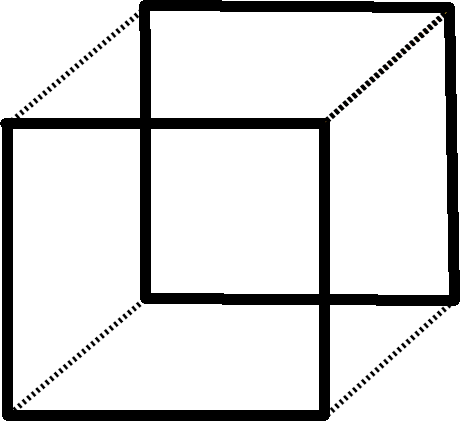
\includegraphics[width=0.9\textwidth]{2023ECRW/Figures/fluidelement.png}
% \begin{itemize}
%     \item Directly modelled
%     \item Kinetic, Magnetic, thermal
% \end{itemize}
% \end{column}
% \begin{column}{0.3\textwidth}
% \centering
% \textbf{Ionisation/excitation energy}
% 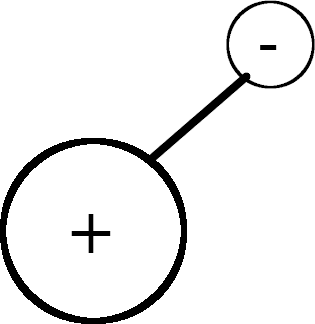
\includegraphics[width=0.8\textwidth]{2023ECRW/Figures/ionenergy.png}
% \begin{itemize}
%     \item Not directly modelled but can be calculated
%     \item Non-conservative 
%     \item Energy remains 'in the system'.
% \end{itemize}
% \end{column}
% \begin{column}{0.3\textwidth}
% \centering
% \textbf{Radiative energy}
% 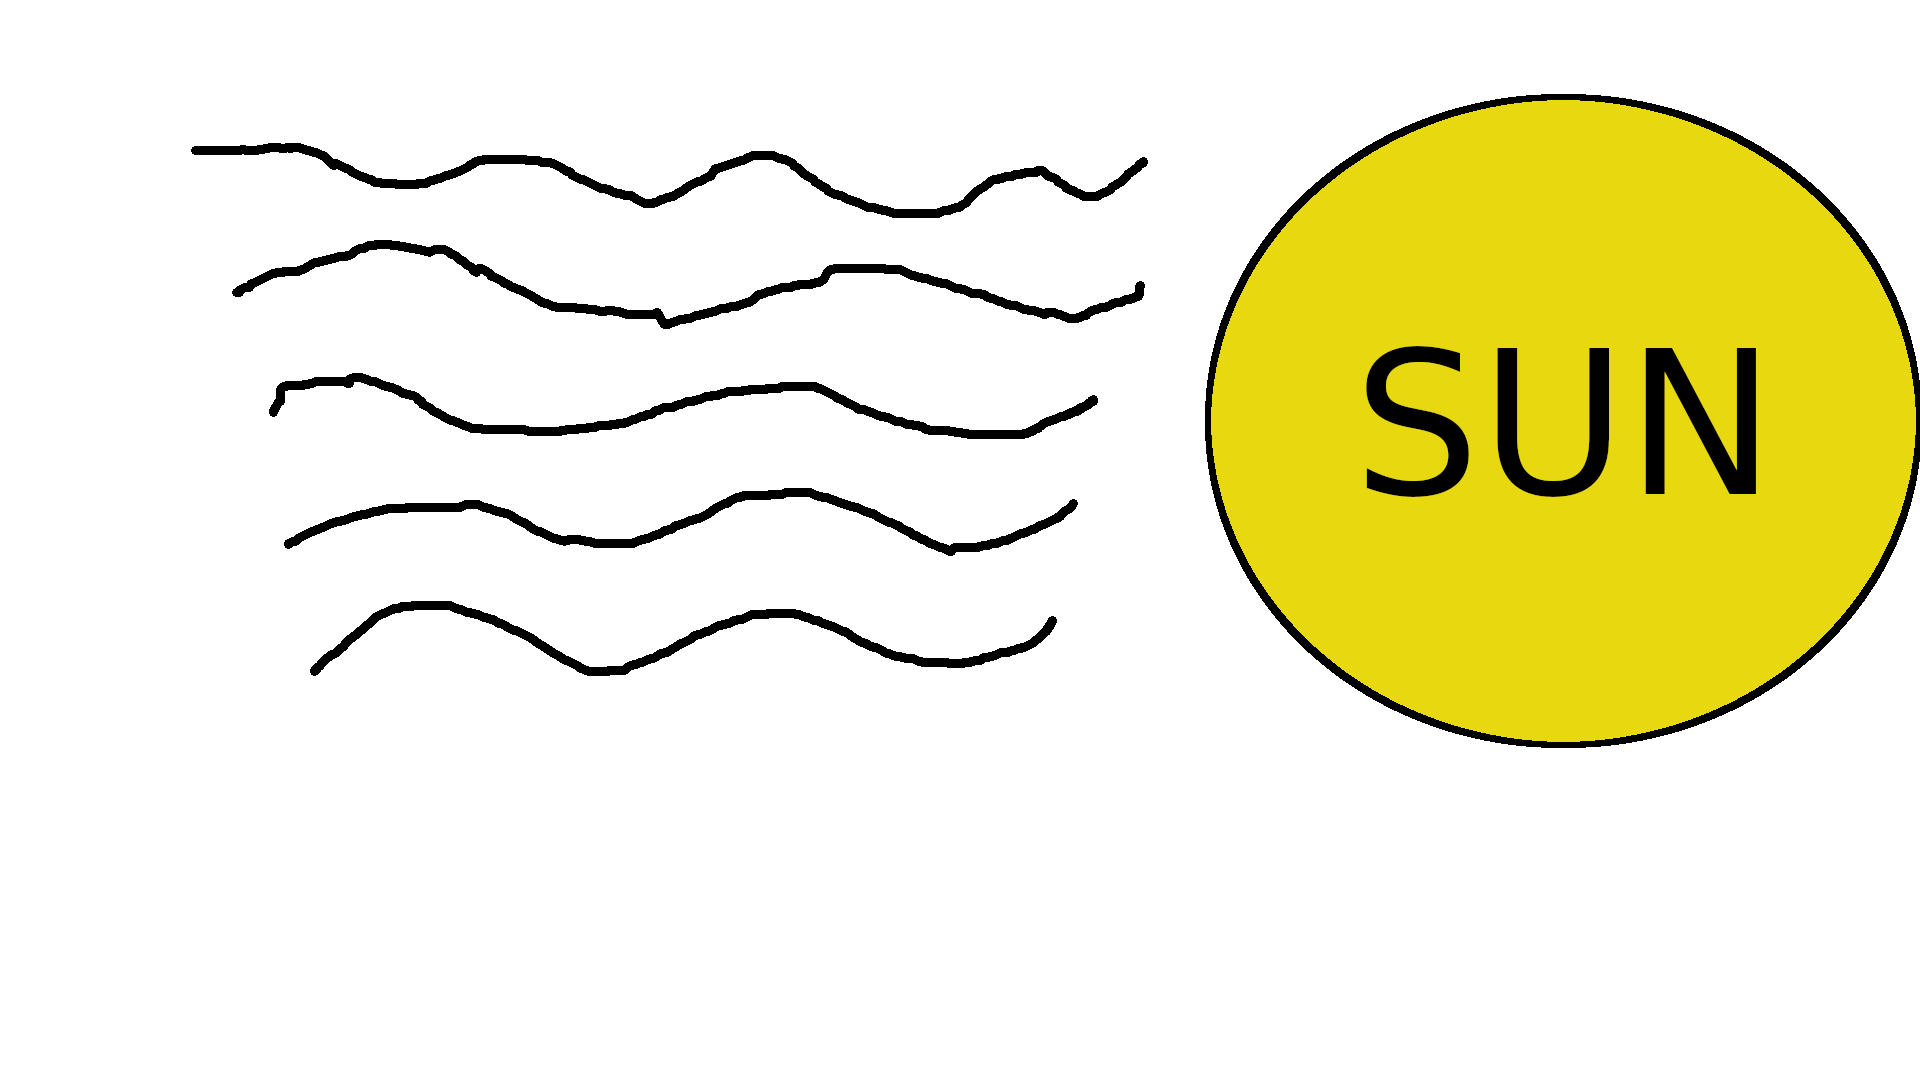
\includegraphics[width=0.8\textwidth, trim=0cm 2cm 0cm 0cm,clip]{2023ECRW/Figures/radiationenergy.png}
% \begin{itemize}
%     \item Blackbody radiation field
%     \item Not directly modelled/calculable 
%     \item Allows energy to leave/enter the system
% \end{itemize}
% \end{column}
% \end{columns}
% \end{frame}

% \begin{frame}{Ionisation energy losses and recombination energy gains}
% \begin{columns}
% \begin{column}{0.4\textwidth}
% \begin{itemize}
%     \item Ionisation potential term: macroscopic energy lost during collisional ionisation. %Requires a heating term to balance.
%     \item Similar heating during collisional recombination.
%     \item Self-consistent heating/cooling mechanism.
%     \item Neutral level populations solved at each time step using excitation/de-excitation rates.
% %    \item We perform 1D two-fluid simulations of ionisation, recombination and ionisation potential terms in a slow-mode shock.
% \end{itemize}
% \end{column}
% \begin{column}{0.6\textwidth}
% \begin{gather}
%     \hat{I}_{\rm ion}= \Sigma \hat{n}_i \hat{C}_{i{\rm p}} E_i \\
%     \hat{I}_{\rm exc}= \Sigma \hat{n}_1 \hat{C}_{1u} (E_u-E_1) + \Sigma \hat{n}_2 \hat{C}_{2u} (E_u-E_2) \nonumber \\
%     \hspace{1cm} + \Sigma \hat{n}_3 \hat{C}_{3u} (E_u-E_3) + \hat{n}_4 \hat{C}_{4,5} (E_5-E_4)  \\
%     \phi_{I}=(\hat{I}_{\rm{ion}}+\hat{I}_{\rm{exc}})/\hat{\phi} 
% \end{gather}
% \begin{gather}
%     \hat{R}_{\rm rec}= \Sigma \hat{n}_{\rm p} \hat{C}_{{\rm p}i} E_i \\
%     \hat{R}_{\rm dex}= \Sigma \hat{n}_5 \hat{C}_{5l} (E_l-E_5) + \Sigma \hat{n}_4 \hat{C}_{l4} (E_l-E_4)  \nonumber \\
%     \hspace{1cm} + \Sigma \hat{n}_3 \hat{C}_{l3} (E_3-E_l) + \hat{n}_2 \hat{C}_{2,1} (E_1-E_2)  \\
%     \phi_{R}=(\hat{R}_{\rm rec}+\hat{R}_{\rm dex})/\hat{\phi} 
% \end{gather}
% \end{column}
% \end{columns}
% \end{frame}

\begin{frame}{Equilibrium}
\begin{itemize}
    \item Everything determined by electron temperature and number density
\end{itemize}
\begin{gather}
    \rho_p \propto n_e \\
    \xi_n=F(T_e,n_e) \xrightarrow{} \rho_n=G(T_e,n_e)
\end{gather}
\begin{itemize}
    \item Therefore, total pressure depends on the reference values either side of the interface
    \item Iterative solver for IC: 1) find equilibrium on one side. 2) specify the desired jump in electron number density. 3) Find what electron temperature satisfies constant pressure
    \item Doesn't work across the smoothed discontinuity.
\end{itemize}
\end{frame}

\begin{frame}{Getting an equilibrium}
\begin{columns}
\begin{column}{0.3\textwidth}
    \begin{itemize}
        \item Lower layer: $T=5500, \rho_p=1,\rho_n \approx 208, \xi_n\approx 0.995$ 
        \item Lower layer: $T\approx 7319, \rho_p=30,\rho_n \approx 97, \xi_n\approx 0.764$ 
    \end{itemize}
\end{column}
\begin{column}{0.7\textwidth}
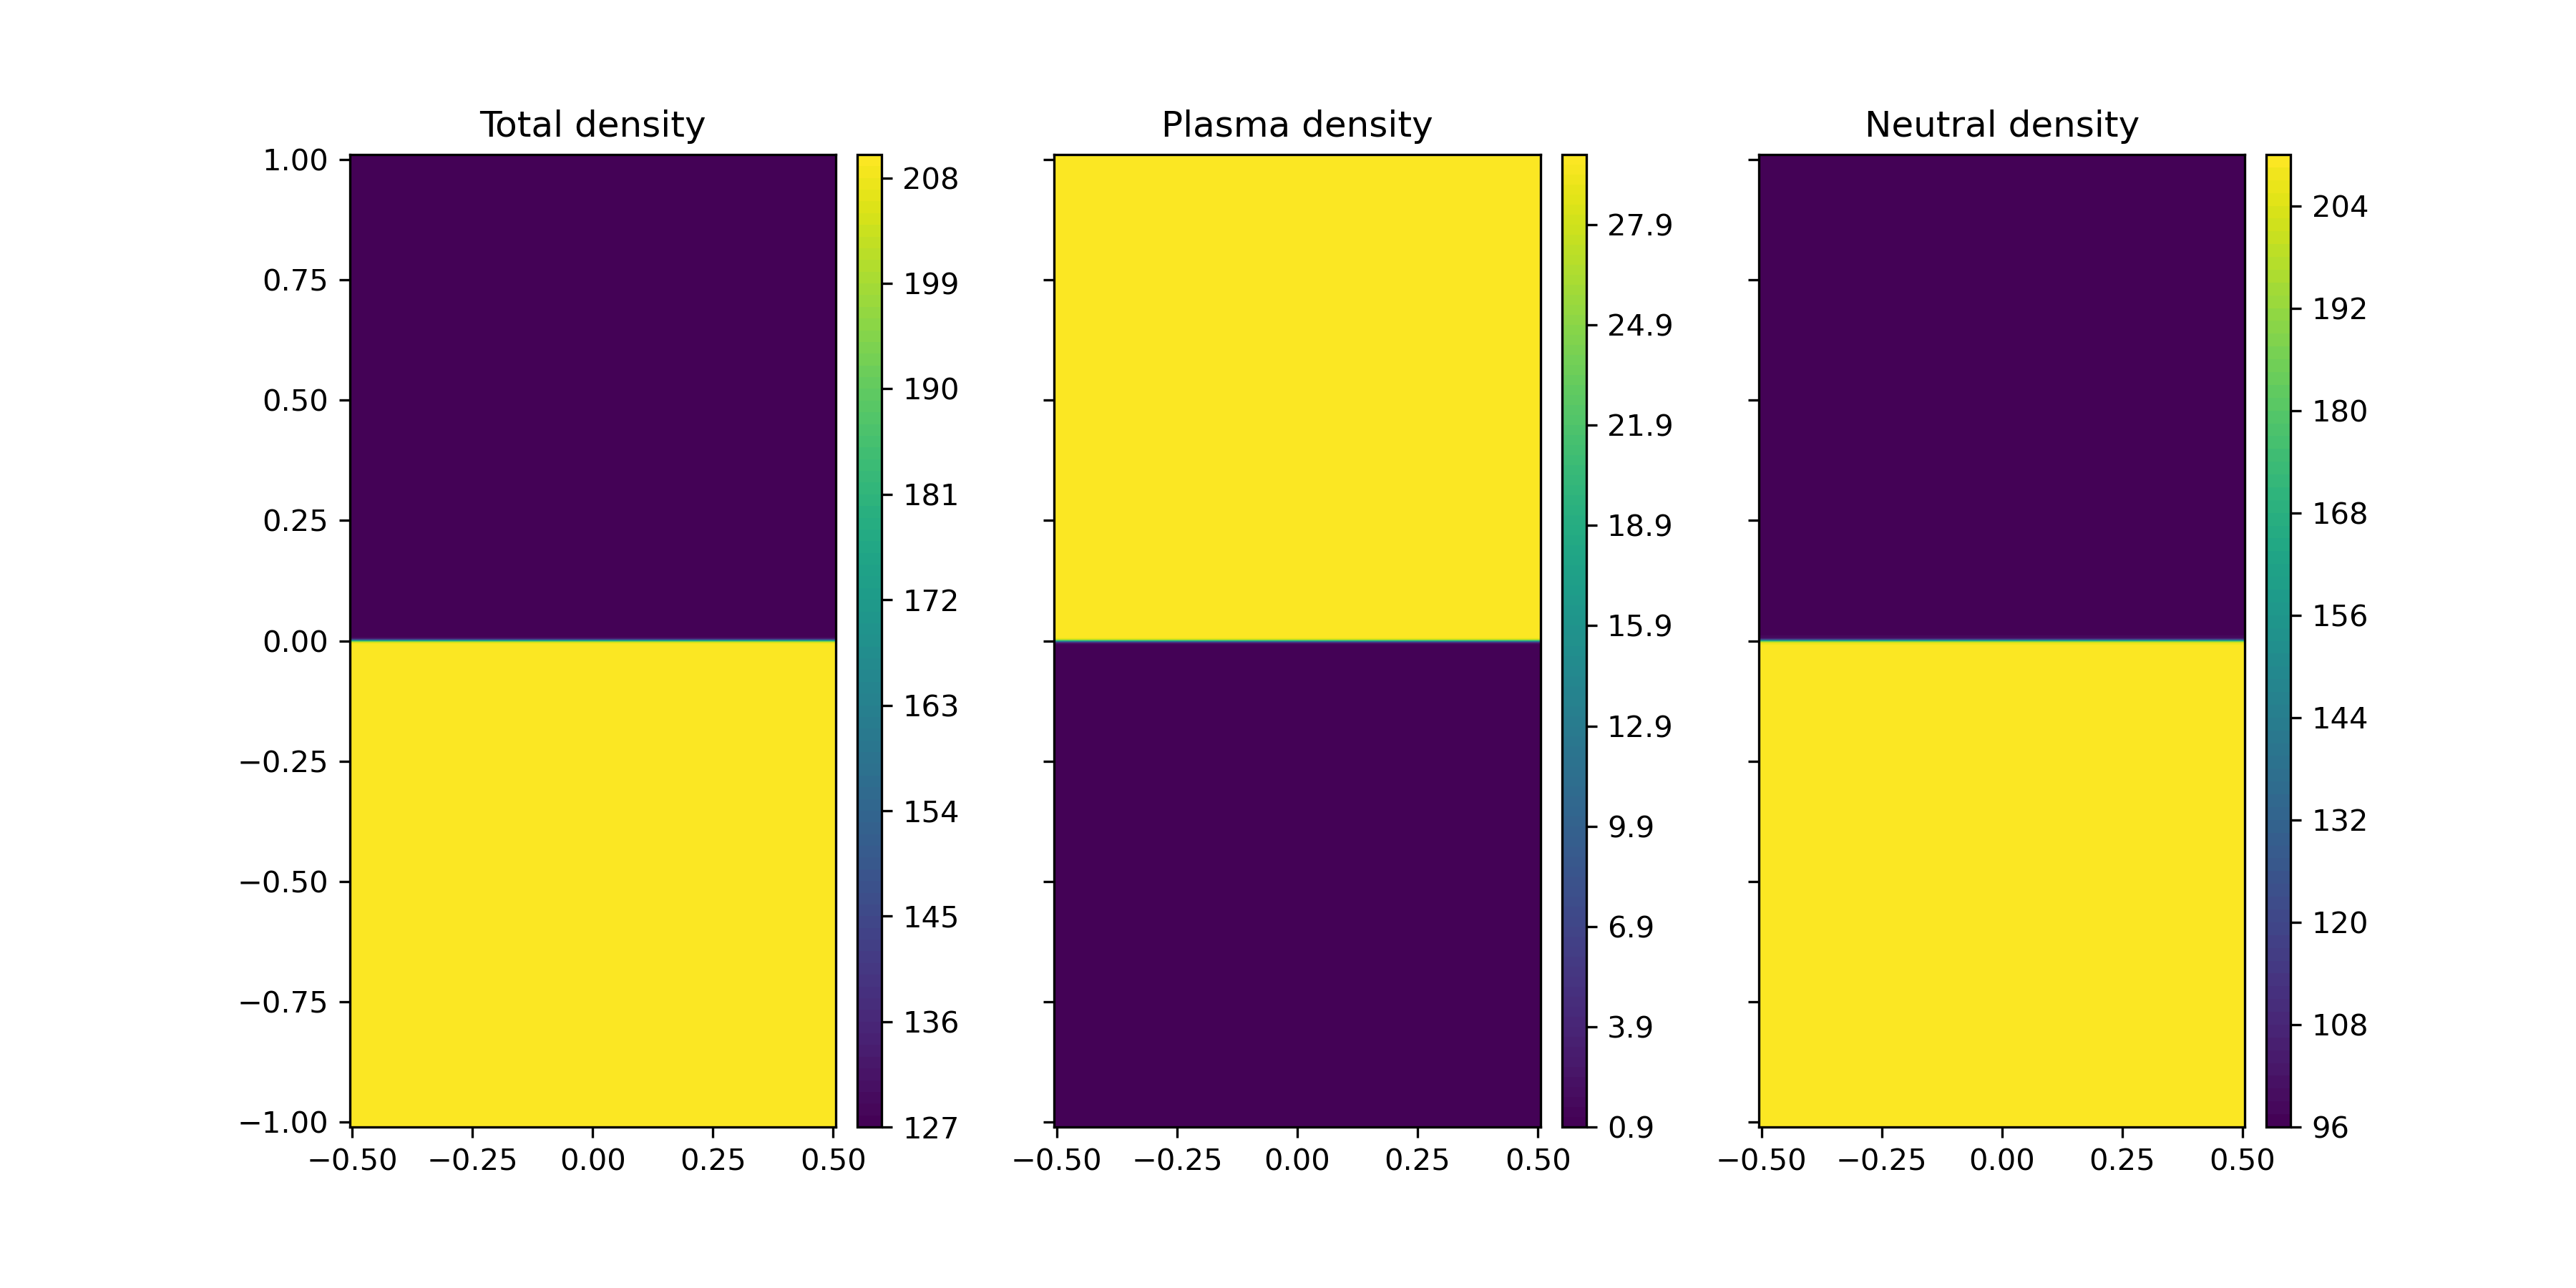
\includegraphics[width=0.99\textwidth]{2023Mixing/Figures/KHInlev_initialconditions.png}
\end{column}
\end{columns}
\end{frame}

% \begin{frame}{Numerical model}
% \begin{columns}
% \begin{column}{0.5\textwidth}
% \begin{enumerate}
% \item KHI mixing
% \end{enumerate}
% \end{column}
% \begin{column}{0.5\textwidth}

% \end{column}
% \end{columns}
% \end{frame}

\begin{frame}{Movie}
\begin{columns}
\begin{column}{0.5\textwidth}
\begin{enumerate}
\item KHI mixing
\end{enumerate}
\end{column}
\begin{column}{0.5\textwidth}

\end{column}
\end{columns}
\end{frame}

\begin{frame}{Snapshot}
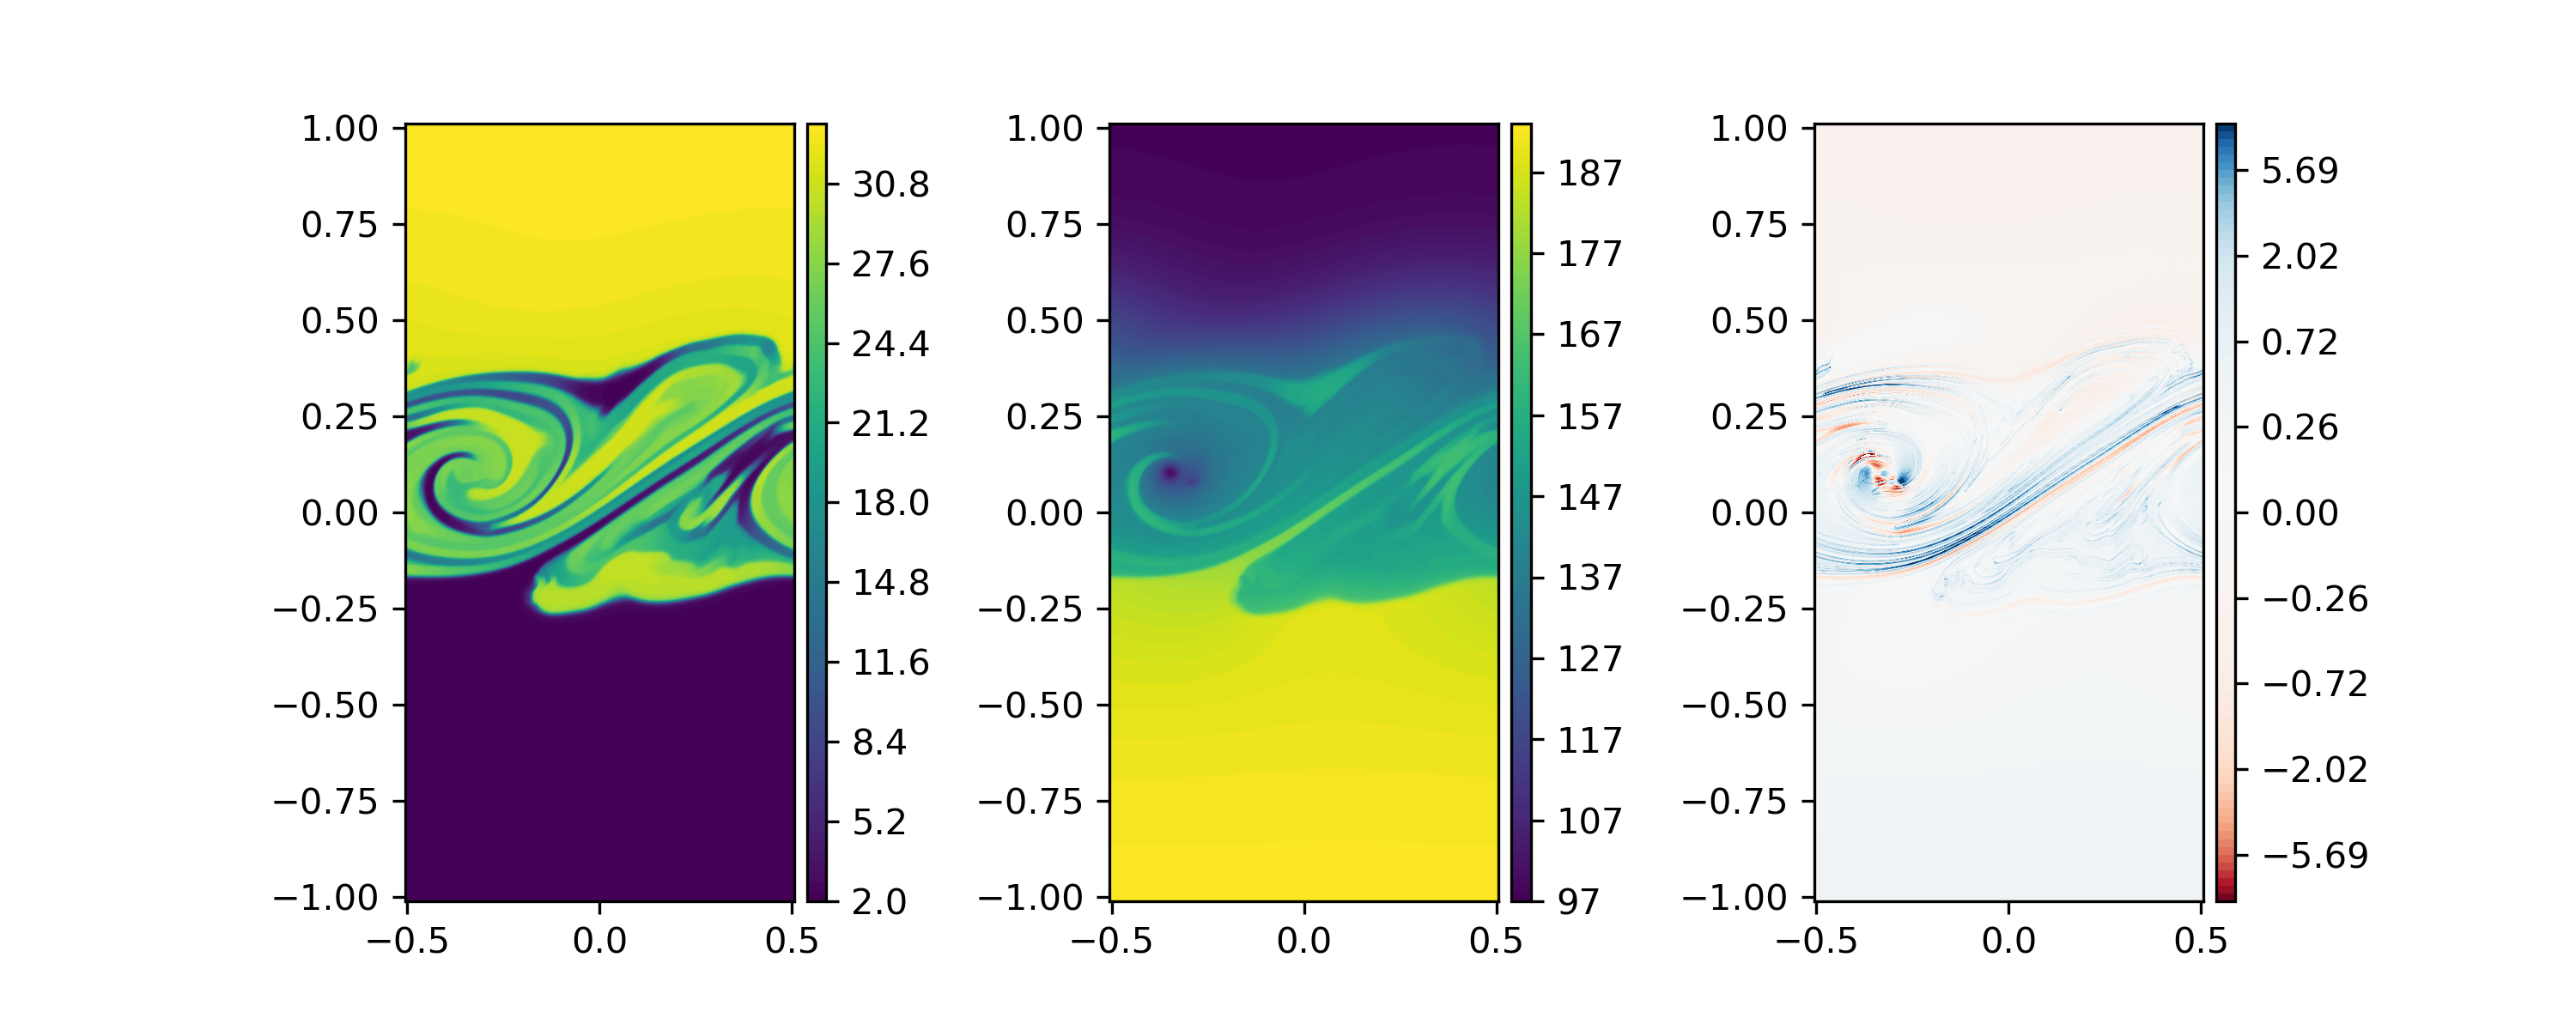
\includegraphics[width=0.99\textwidth]{2023Mixing/Figures/KHInlev_testplot2.png}
\end{frame}

\begin{frame}{Width tests}
\begin{columns}
\begin{column}{0.5\textwidth}
\begin{enumerate}
\item Use width arguments from Hillier's talk
\item Densities normalised to 1
\item Fits reasonable well - mixing layer contained within the widths
\end{enumerate}
\end{column}
\begin{column}{0.5\textwidth}
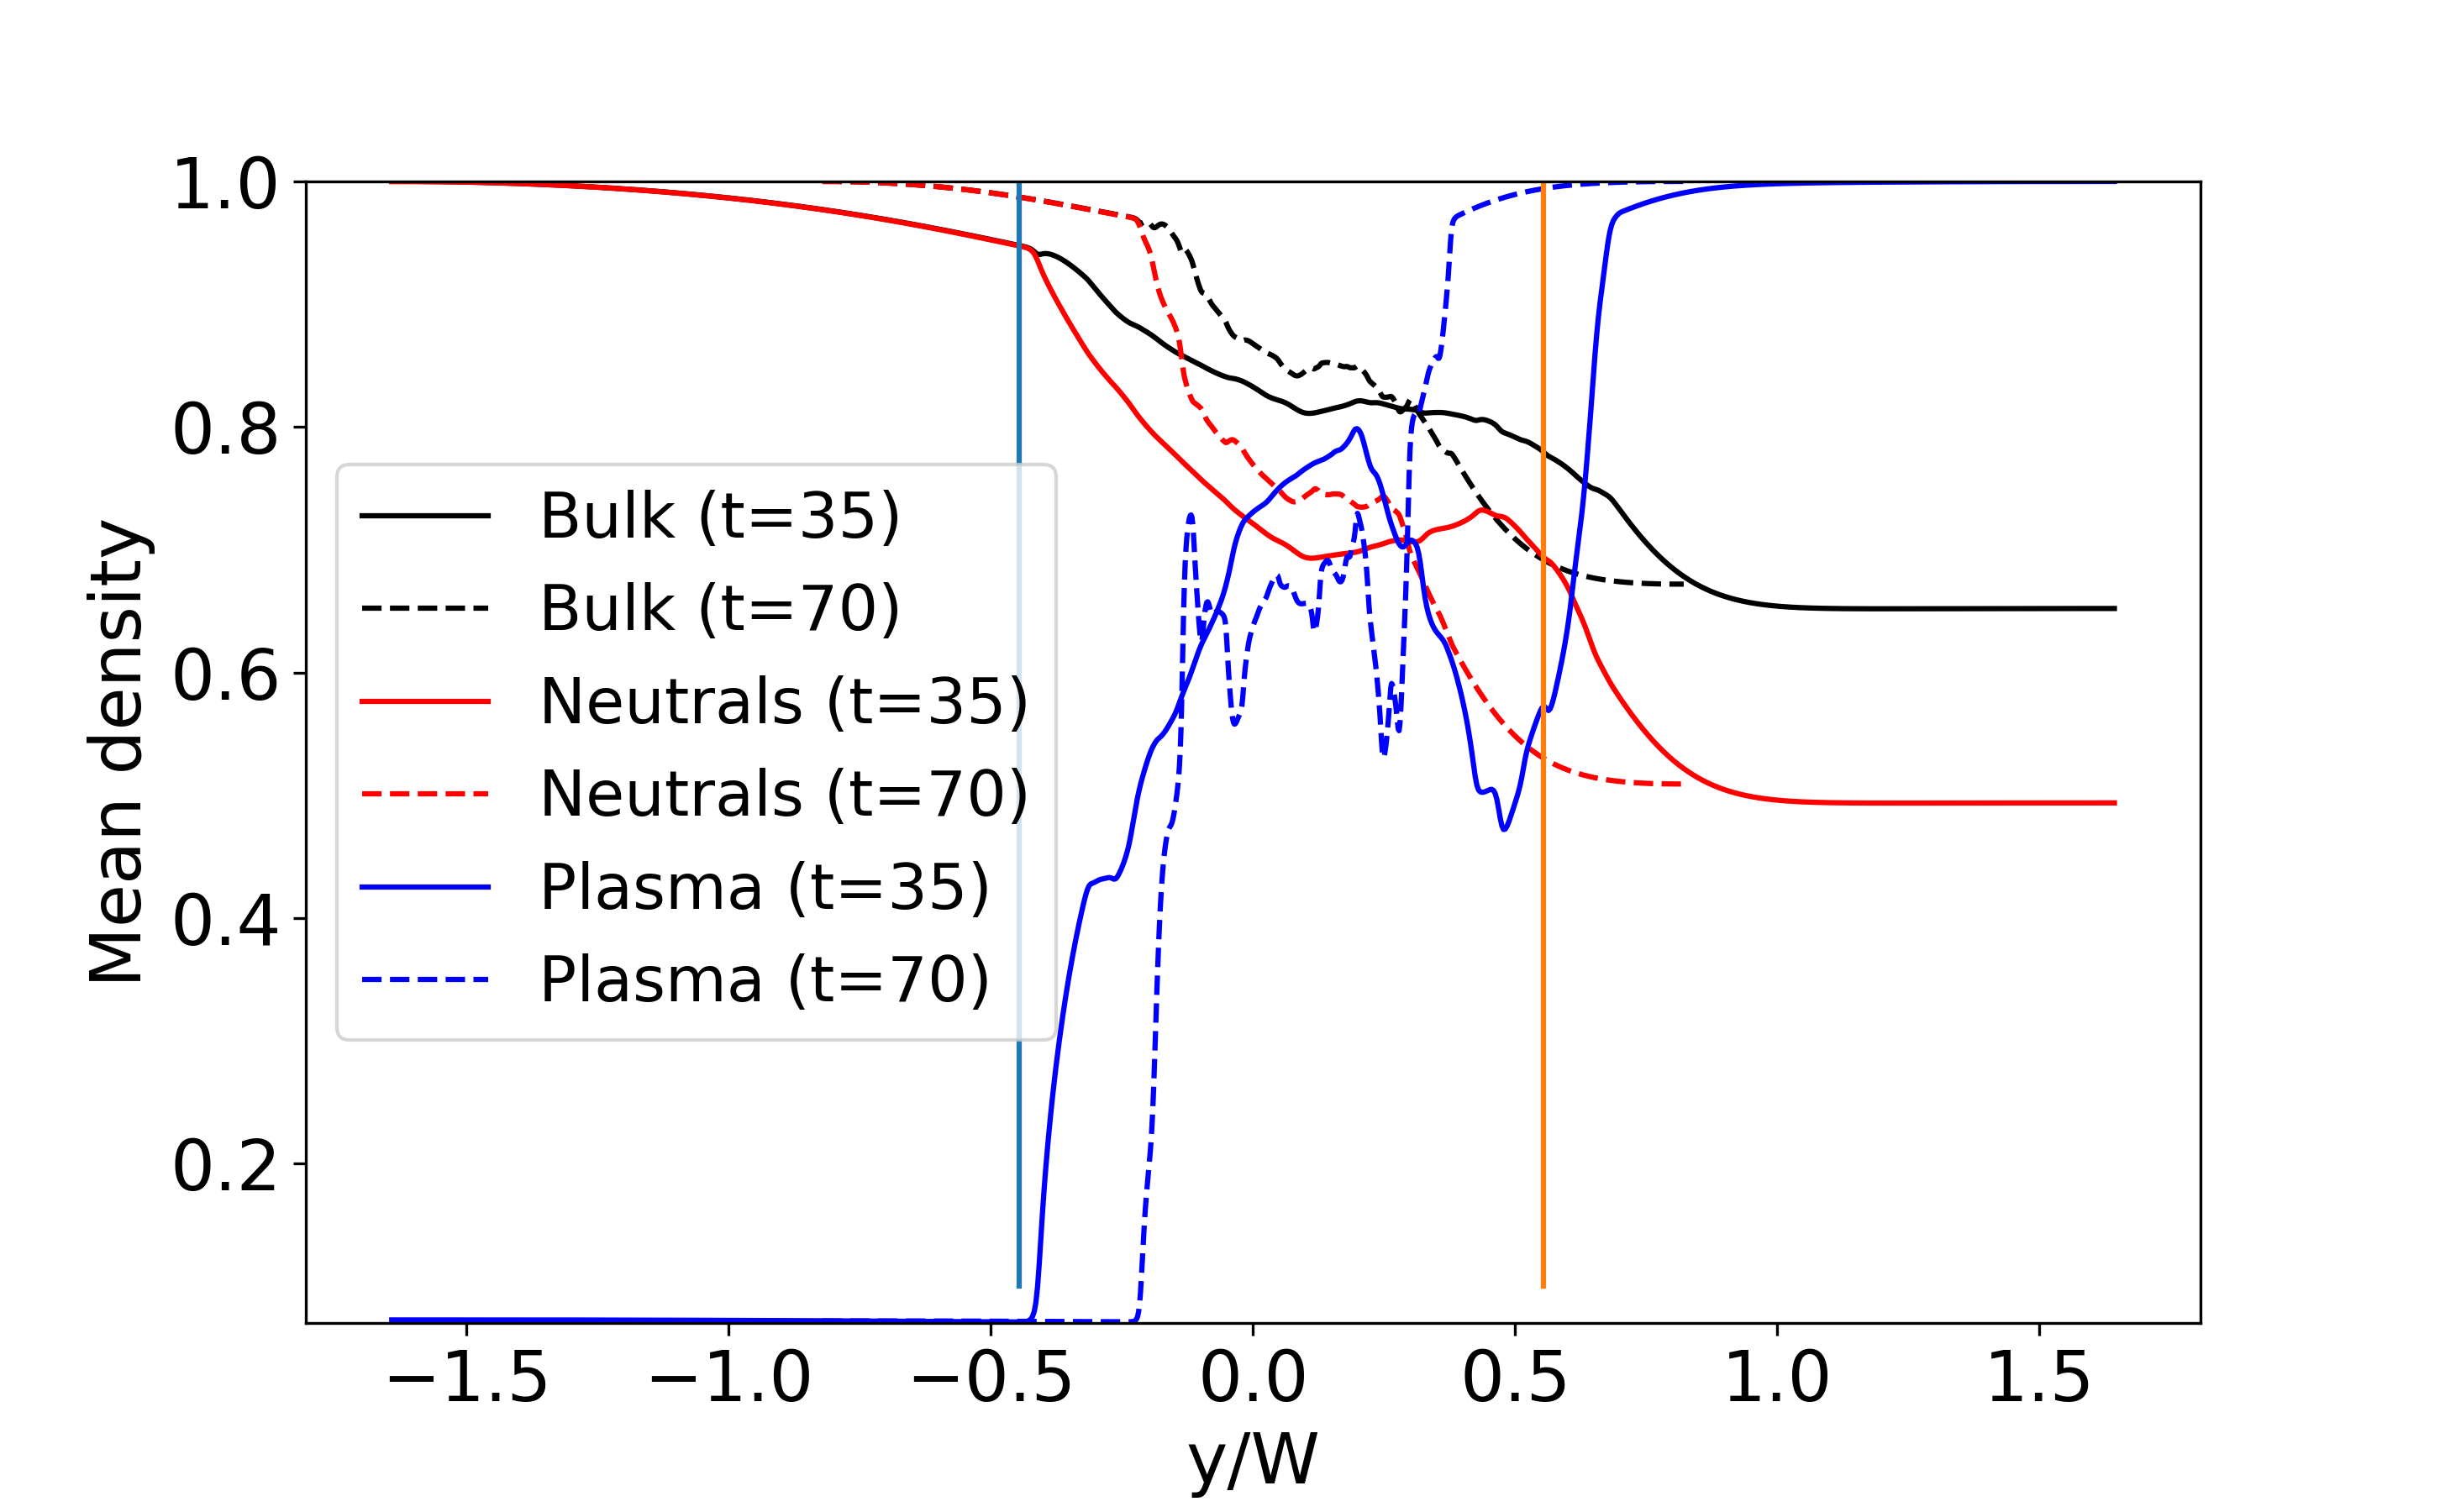
\includegraphics[width=0.99\textwidth]{2023Mixing/Figures/KHInlev_widthtest.png}
\end{column}
\end{columns}
\end{frame}

\begin{frame}{Losses/heating within the system}
\begin{columns}
\begin{column}{0.5\textwidth}
\begin{enumerate}
\item Total losses within the mixing layer
\item Overall, heating greater than cooling
\item System mixes to lower mean temperature 
\item Lower mean ion fraction
\item Collisional only so heating during recombination/de-excitation
\end{enumerate}
\end{column}
\begin{column}{0.5\textwidth}
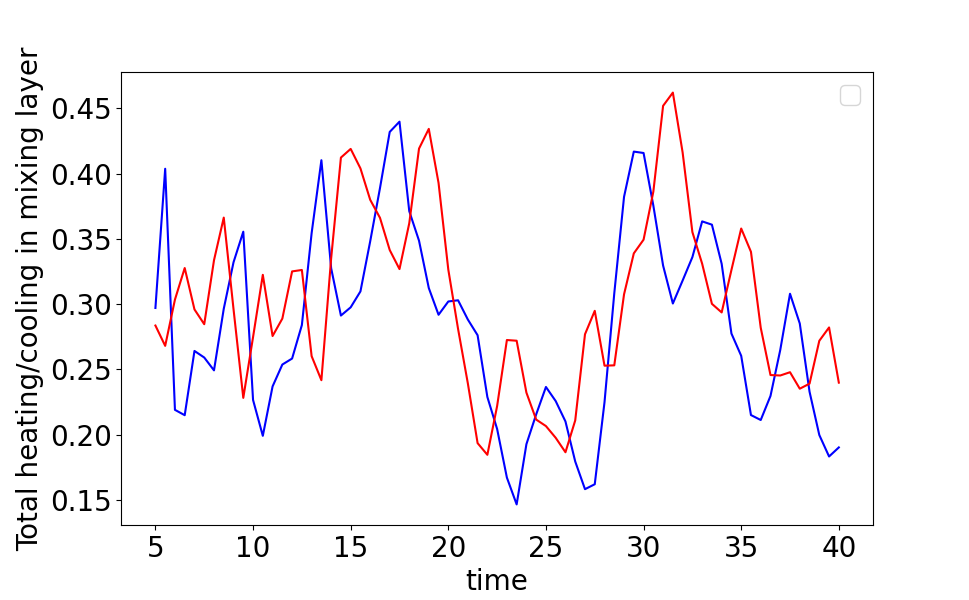
\includegraphics[width=0.99\textwidth]{2023Mixing/Figures/KHInlev_losstimeplot.png}
\end{column}
\end{columns}
\end{frame}

\begin{frame}{Conclusions}
\begin{itemize}
    \item KHI-mixing in partially ionised plasma (out of plane magnetic field)
\end{itemize}
\end{frame}

% \begin{frame}{Populations at different heights}
% \begin{columns}
% \begin{column}{0.5\textwidth}
% \begin{figure}
%     \centering
% %\includegraphics[width=0.95\linewidth,clip=true,trim=0.9cm 7.8cm 1.5cm 7.8cm]{figures/widthradt2_sw.pdf}
% %    \caption{Finite width of the shock as a function of upstream recombination rates.}
%     \includegraphics[width=0.95\linewidth]{2023RAS/Figures/saha2_plot.png}
%     \caption{Temperature (red) and ion fraction through height (using VALCIII data)}
%     \label{fig:shockwidthsw}
% \end{figure}
% \end{column}
% \begin{column}{0.42\textwidth}
% \begin{itemize}
%     \item Different atmospheric heights have different temperatures and electron number densities.
%     \item Different importance of radiative/collisional rates
%     \item Sample a few heights
% \end{itemize}
% \end{column}
% \end{columns}
% \end{frame}

% \begin{frame}{Numerical simulation - mid chromosphere}
% \begin{columns}
% \begin{column}{0.8\textwidth}
% \begin{figure}
%     %\centering
%     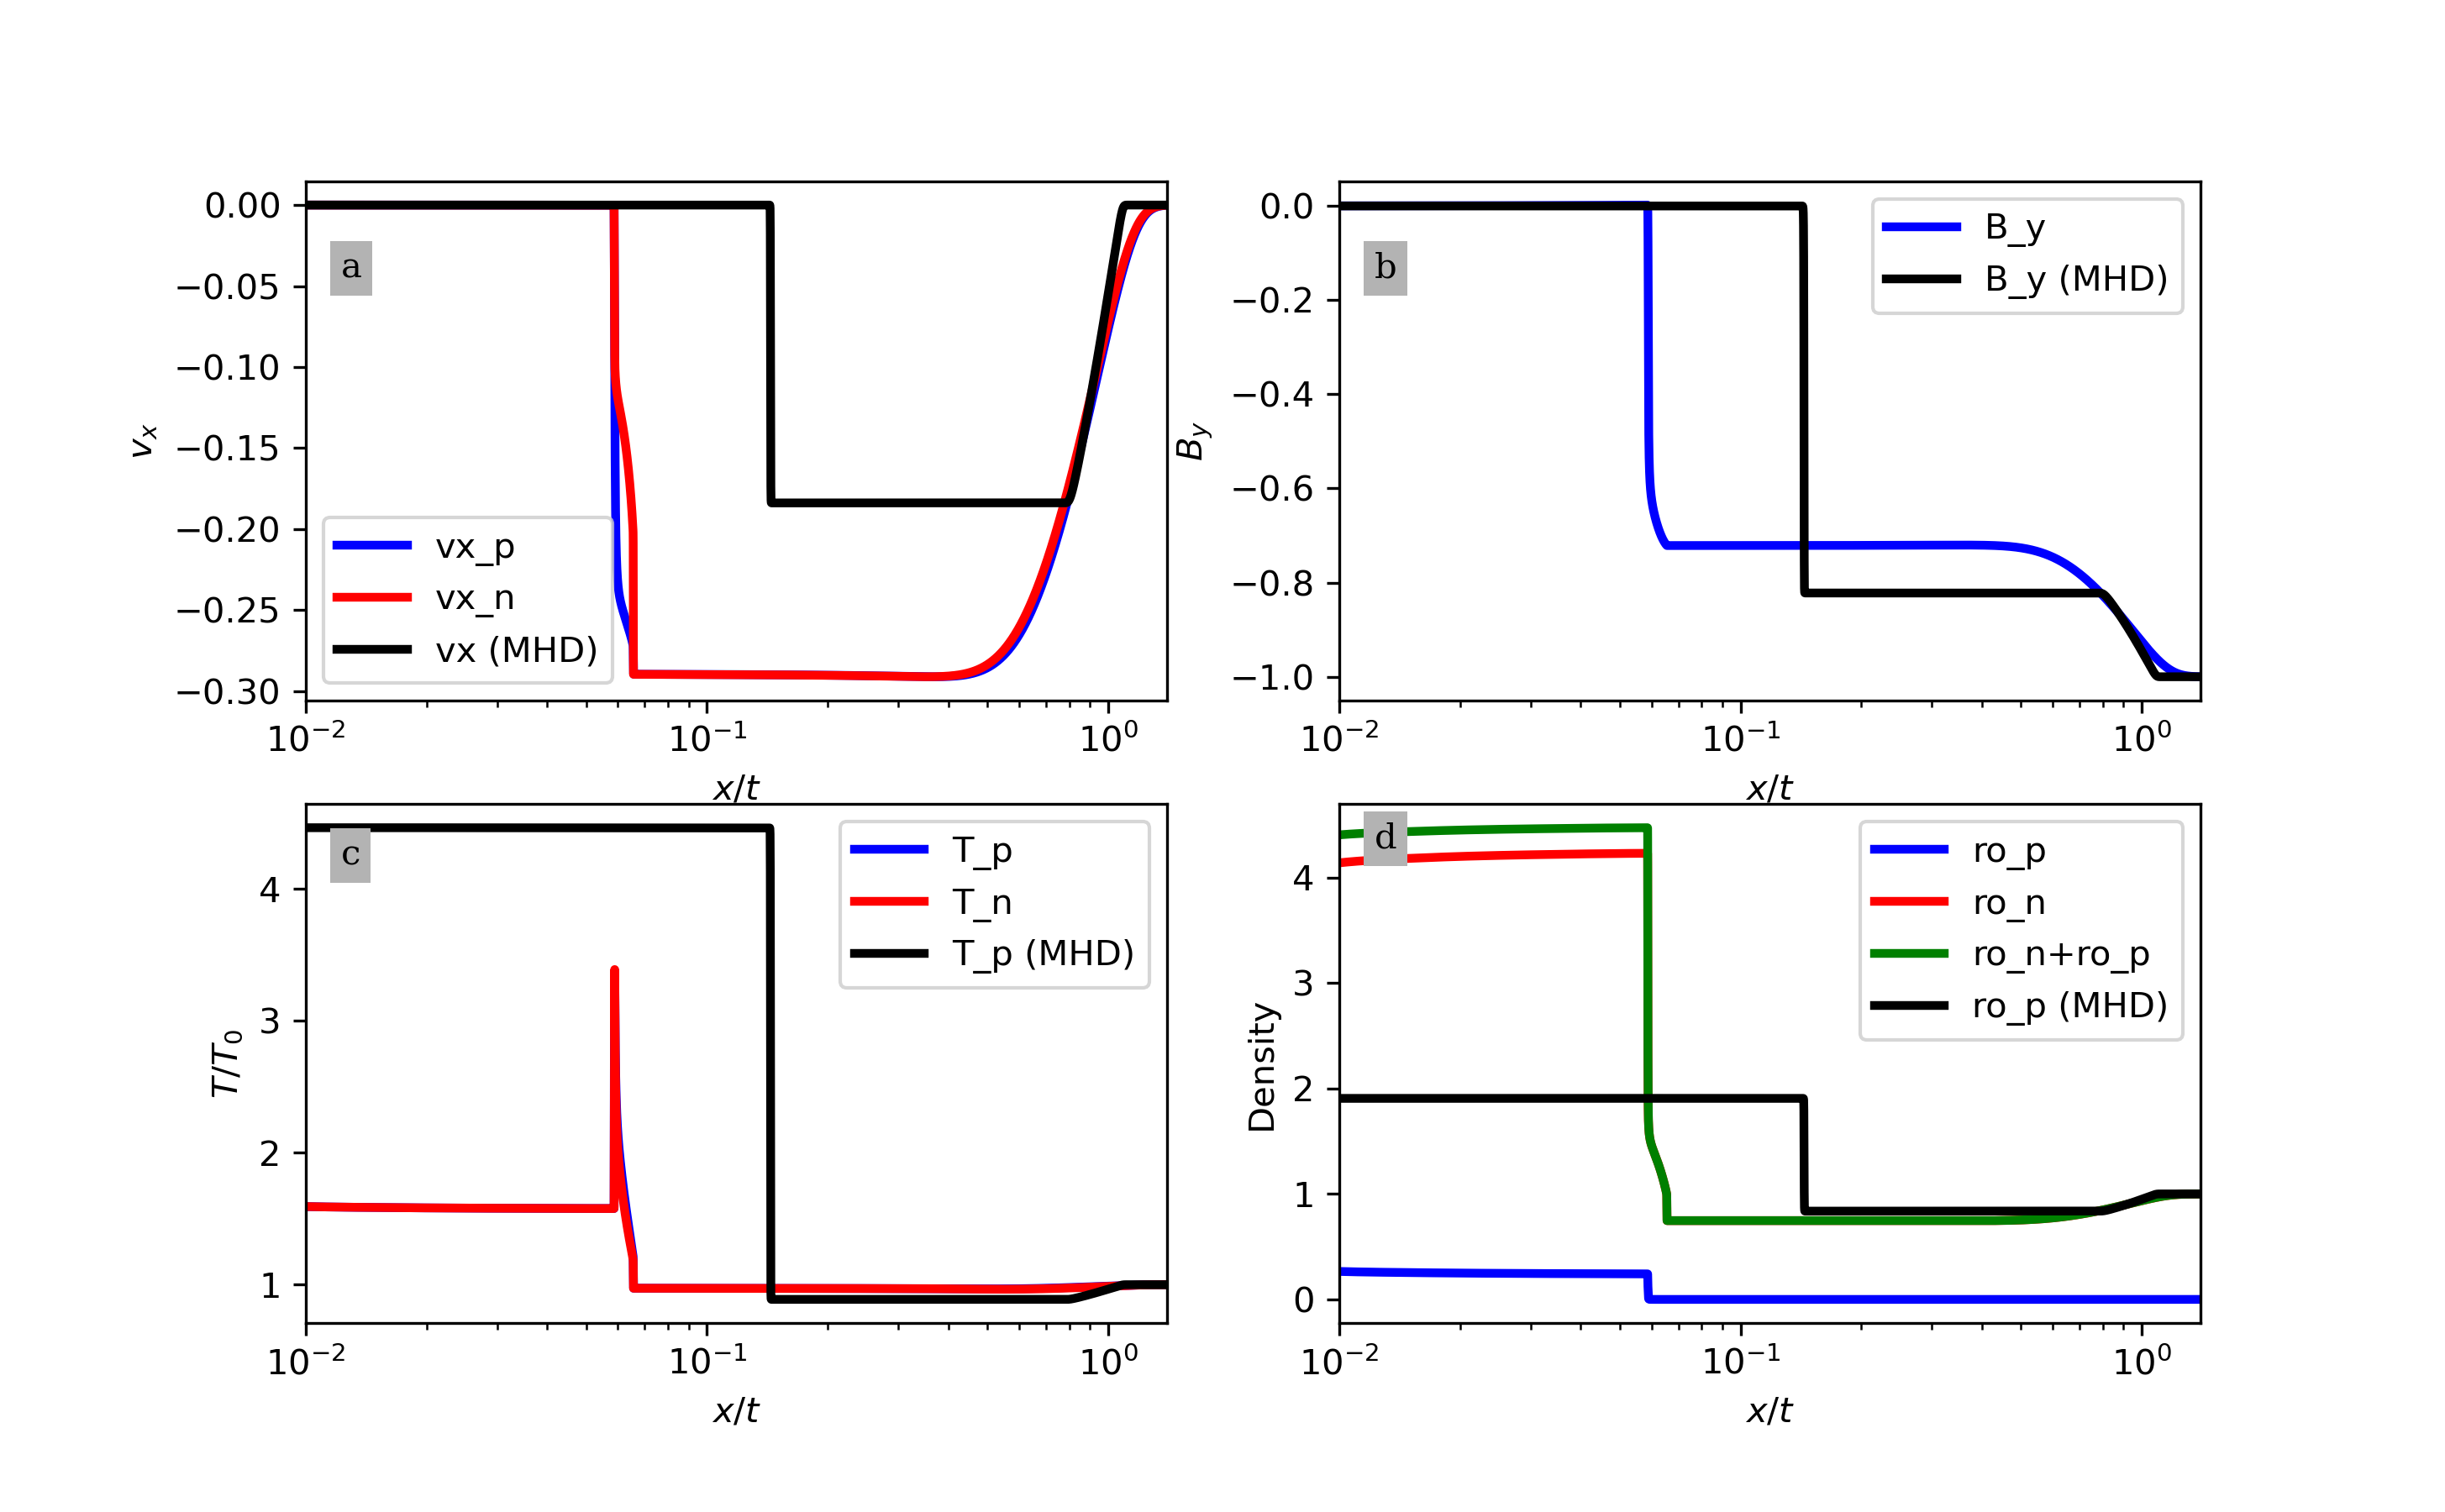
\includegraphics[width=0.95\linewidth,clip=true,trim=0.9cm 0.8cm 0.9cm 0.8cm]{Figures/context_midc.png}
%     %\caption{Upper-chromosphere case showing the $v_x$ velocity (top left), $B_y$ magnetic field (top right), temperature (lower left) and density (lower right). For panel c, the reference temperature $T_0=6220$.}
%     \label{fig:midchromocontext}
% \end{figure}
% \end{column}
% \begin{column}{0.2\textwidth}
% %\begin{itemize}
%     $T_0=5030$, $n_e=7.5\times 10^{16}$, $\xi_n=0.9997$
% %\end{itemize}
% \end{column}
% \end{columns}
% \end{frame}

% \begin{frame}{Shock substructure - mid chromosphere}
% \begin{columns}
% \begin{column}{0.8\textwidth}
% \begin{figure}
%     %\centering
%     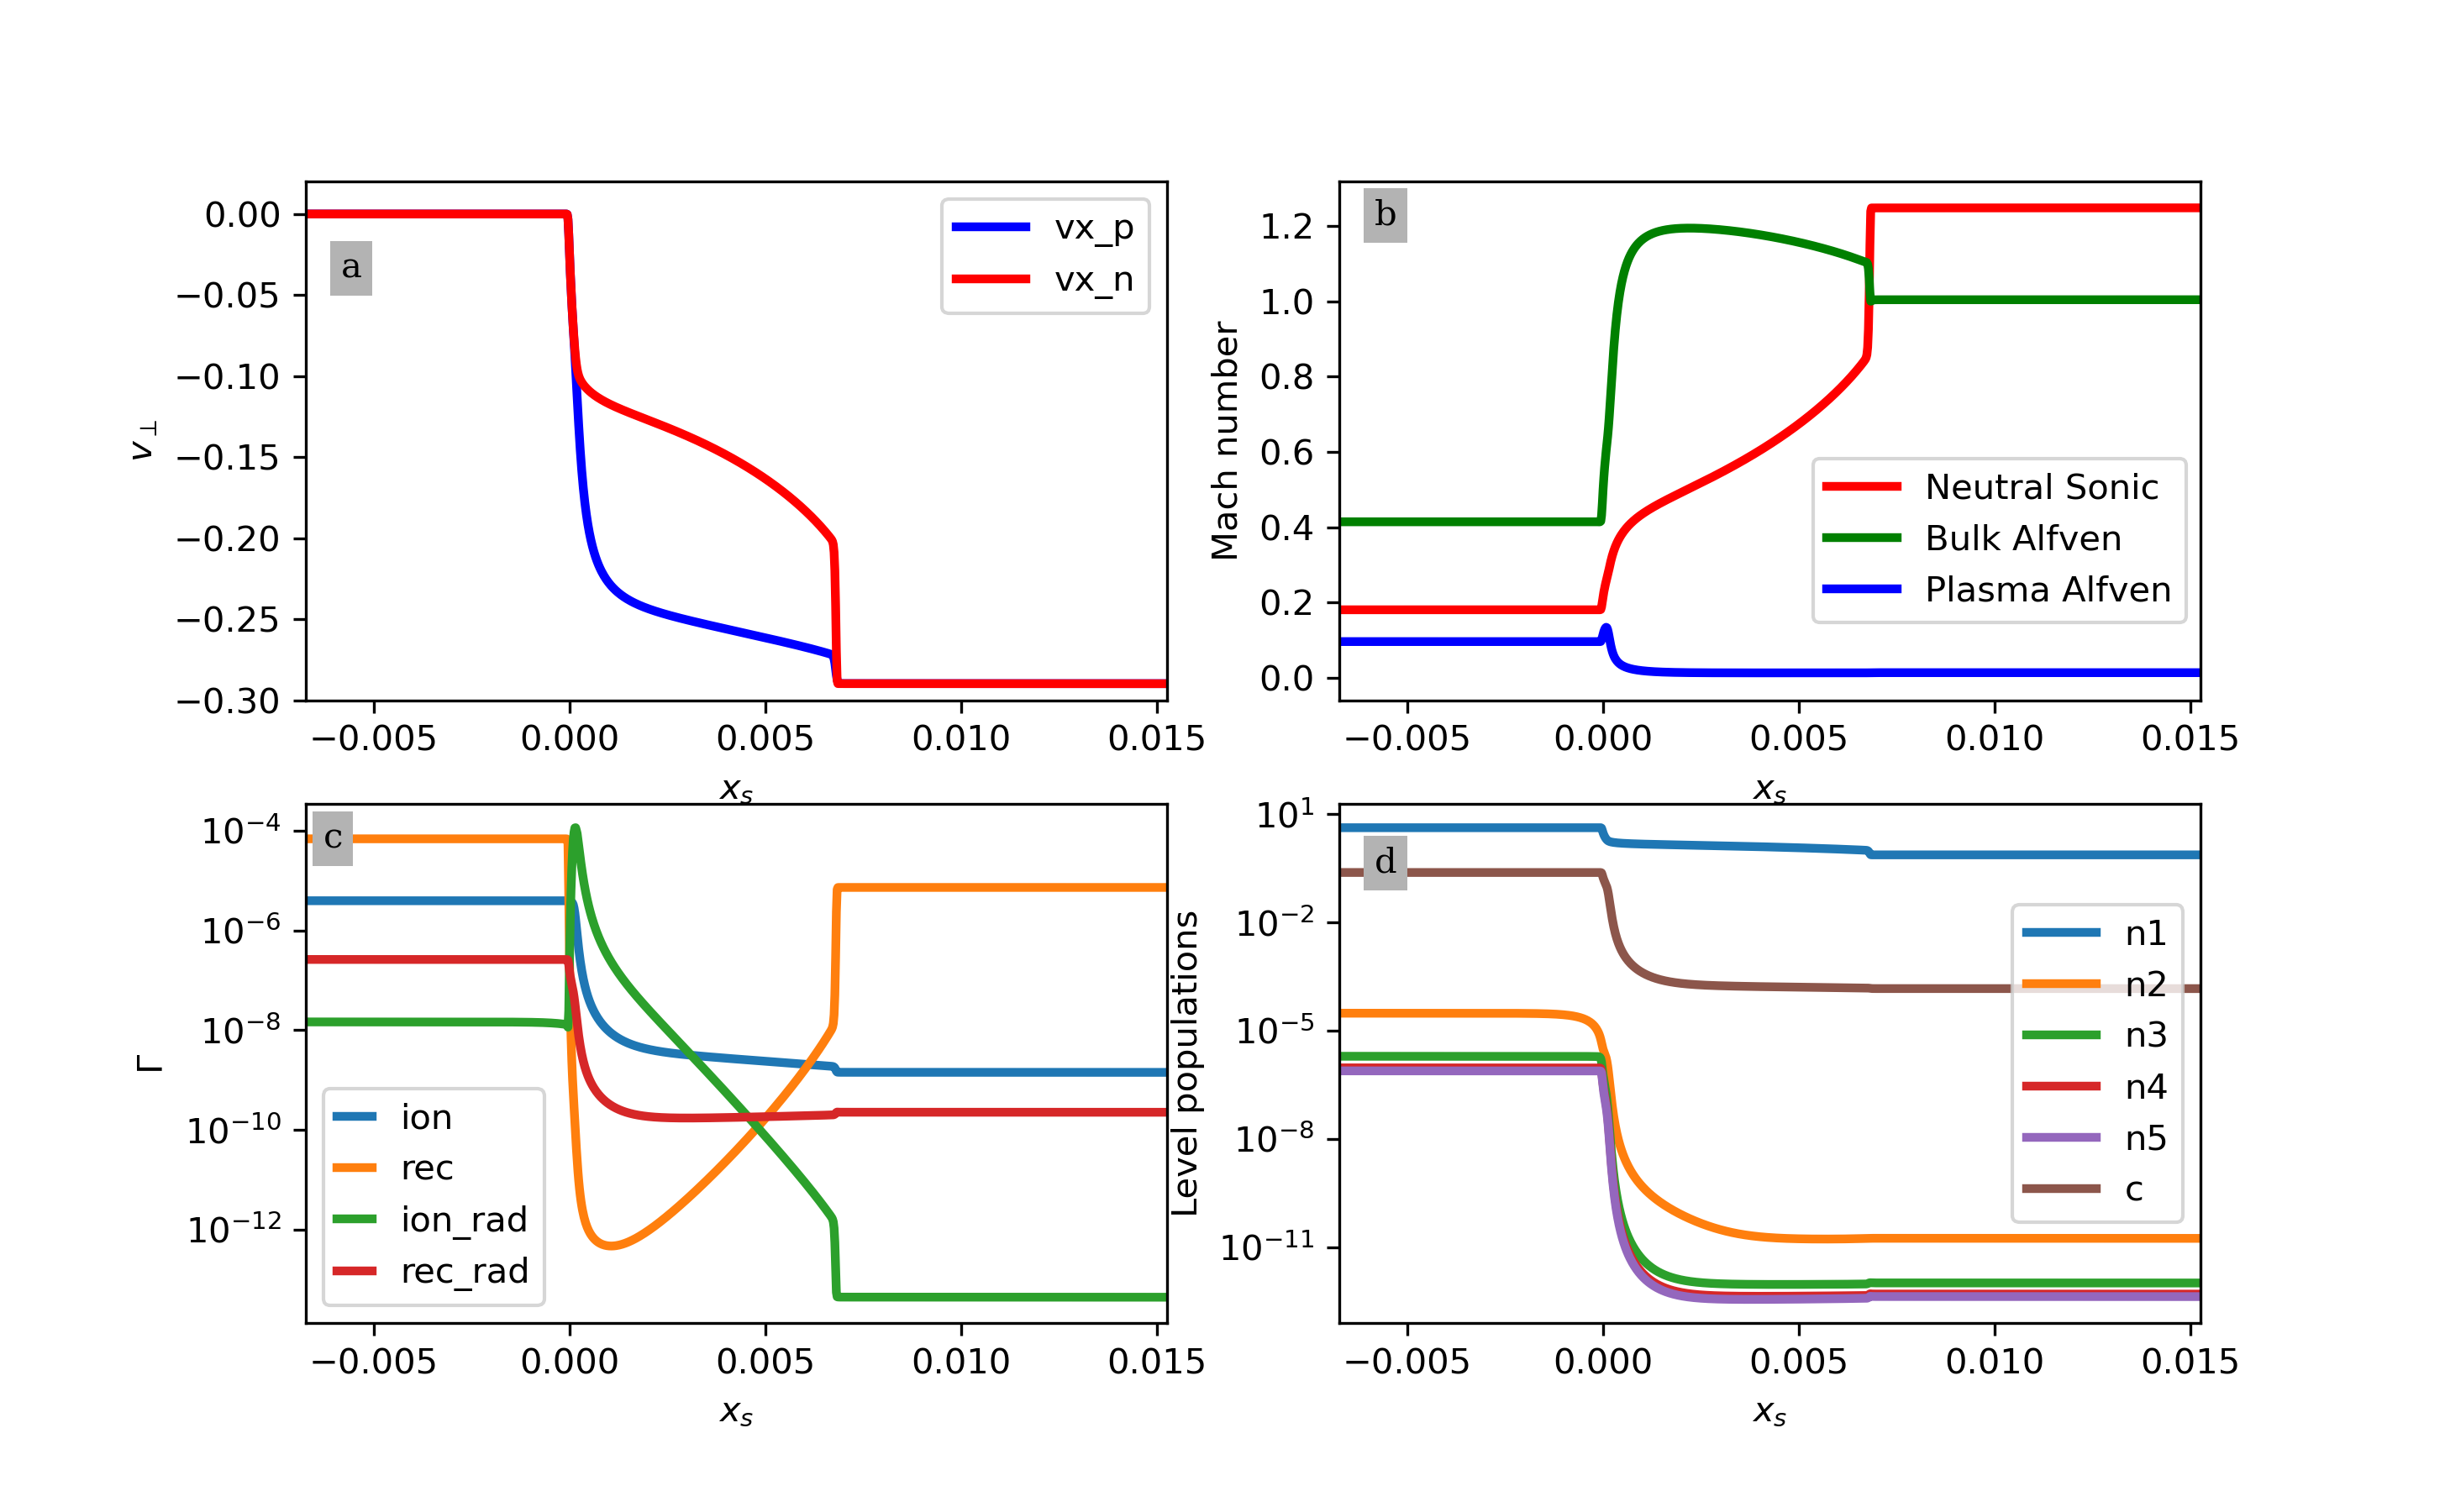
\includegraphics[width=0.9\linewidth,clip=true,trim=1.2cm 0.8cm 0.9cm 0.8cm]{Figures/shocksub2_plot_midc.png}
%     %\caption{Upper-chromosphere case showing the $v_x$ velocity (top left), $B_y$ magnetic field (top right), temperature (lower left) and density (lower right). For panel c, the reference temperature $T_0=6220$.}
%     \label{fig:midchromocontext}
% \end{figure}
% \end{column}
% \begin{column}{0.2\textwidth}
% %\begin{itemize}
%     $T_0=5030$, $n_e=7.5\times 10^{16}$, $\xi_n=0.9997$
% %\end{itemize}
% \end{column}
% \end{columns}
% \end{frame}

\end{document}
